% \documentclass[dvipdfmx,b5paper]{skreport}
\documentclass[dvipdfmx]{skreport}
\usepackage{graphics}
\usepackage{amsmath}
\usepackage{amssymb}
\usepackage{amsthm}
\usepackage{mathtools}
\usepackage{ascmac}
\usepackage{bm}
\usepackage{url}
\usepackage{txfonts}
\usepackage{color}
\usepackage{tikz}
\usepackage{docmute}    %パッケージのダウンロードが必要
\usepackage{tikz}
\usetikzlibrary{calc}
\usetikzlibrary{intersections}


\usepackage[dvipdfmx]{hyperref}
\usepackage{pxjahyper}

\newcommand{\mmm}{\hspace{3mm}}
\newcommand{\veczero}{$\vec{0}$}
\newcommand{\veca}{$\vec{a}$}
\newcommand{\vecb}{$\vec{b}$}
\newcommand{\veco}{$\vec{o}$}
\newcommand{\vecx}{$\vec{x}$}
\newcommand{\vecy}{$\vec{y}$}
\newcommand{\vecz}{$\vec{z}$}
\newcommand{\vecrm}[1]{$\overrightarrow{\mathrm{ #1 }}$}
\newcommand{\vecins}[1]{$\vec{#1}$}
\newcommand{\mathins}[1]{${#1}$}

%ページ番号を消す
% \pagestyle{empty}
% \thispagestyle{empty}


\title{数学B:ベクトル}
% \author{近藤 綜太\\s.kondo11235813@gmail.com}
% \date{}



\begin{document}
\maketitle
    高校数学の中でも唯一独立した単元であるベクトルの抽象的な理解を目標とする.\\
    \tableofcontents
    \newpage
    \chapter{ベクトル入門}
    この章ではベクトルの算術的な計算に的を絞り,ベクトルの定義やベクトルの表現,計算について扱う.この章での問題意識はベクトルを今まで通りの文字式計算に直せないのかということだ.
    % \documentclass{jsarticle}
% \usepackage[dvipdfmx]{graphics}
% \usepackage{amsmath}
% \usepackage{amssymb}
% \usepackage{ascmac}
% \usepackage{bm}
% \usepackage{url}
% \usepackage{txfonts}
%
% \newcommand{\mmm}{\hspace{3mm}}
% \newcommand{\veczero}{$\vec{0}$}
% \newcommand{\veca}{$\vec{a}$}
% \newcommand{\vecb}{$\vec{b}$}
% \newcommand{\veco}{$\vec{o}$}
% \newcommand{\vecx}{$\vec{x}$}
% \newcommand{\vecy}{$\vec{y}$}
% \newcommand{\vecz}{$\vec{z}$}
%
%
%
%
% \begin{document}

    \section{ベクトルの定義}
    \subsection{教科書的理解}
    多くの教科書に"ベクトルとは,大きさと向きを持った量"という説明がある.図\ref{fig:vector_yukosenbun}のようなものだろう.矢印の長さが大きさを,さす方向が向きを表している.有向線分という表現も一度は目にしたことがあるだろう.
    %
    \begin{figure}[htbp]
        \begin{center}
            \resizebox{!}{4cm}{
            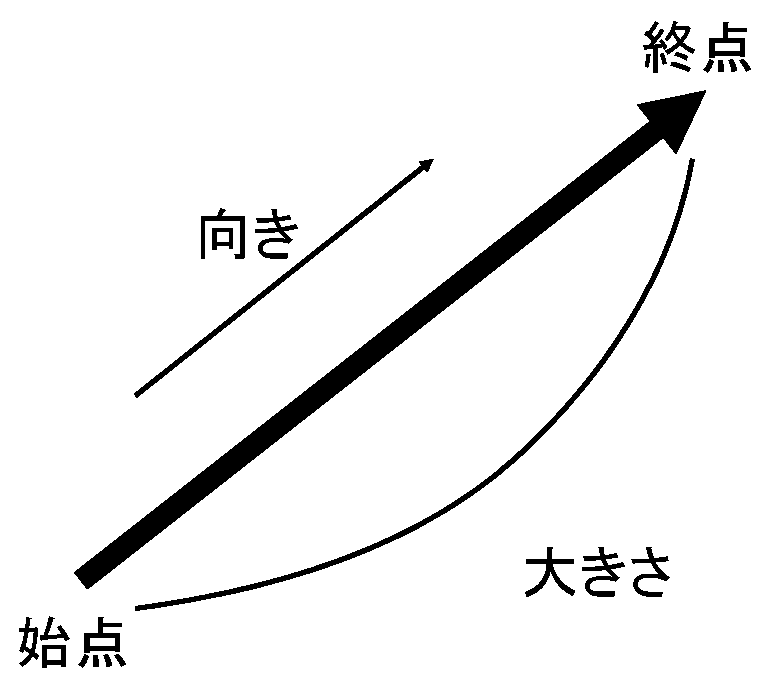
\includegraphics{img/vector_yukosenbun.eps}
            }
        \end{center}
        \caption{有向線分}
        \label{fig:vector_yukosenbun}
    \end{figure}

    今まで意識せずに扱ってきた数値というものは,向きのない大きさだけの量で"スカラ"と呼ばれる.計算では主にこのスカラ量を用いている.いや,計算で主にスカラ量を使っているのではなく,スカラ量であれば計算できるのだ.

    ベクトルの計算を考えたとき,その大きさを扱うのはそれほど難しくはないことが想像できる.これは大きさが数値,すなわちスカラ量であることが理由だ.では向きの計算はどうか.これが問題なのだ.向きといったものは数値として表現するのは簡単ではない.角度を使うことを考えることはできるが,これは数3において扱う極座標,さらには複素数平面で扱う事柄であってそこそこ難しい.

    ベクトルは向きのある量を扱う計算として,この計算が容易ではない"向き"という要素を上手に解決している.

    このような問題意識のもと,次へ進む.

    \subsection{2種のベクトル}
    すでに勉強したのであればベクトルと一口に言っても大きく2つの種類があったと思われる.まず1つ目に挙げられるのは
    \[
    \vec{a},\vec{b},\cdots
    \]
    というように矢印を頭にのせてベクトルを表現と,
    \[
    (1,0),(3,2),\cdots
    \]
    というようにあたかも座標のようにベクトルを表しているものである.この両者は先の問題意識として挙げた向きは計算できないという数学上の問題を解決している.

    ベクトルの問題を解く際にこの2つの違いは解答の方針に大きな差を生むので,同じベクトルの問題という一つのまとまりだという認識ではなく,$\vec{a},\cdots$を使うベクトルの問題,$(1,0),\cdots$を使うベクトルの問題,と分けて理解することを勧める.

    両者の独立した理解が,それらの併用という新たな選択肢を生む.両者の違いを意識して学習しよう.

    \section{$\vec{a}$のようなベクトル}
    文字に矢印をつけてベクトルを表現している.これは大きさ,向きの1セットを1つの記号$\vec{a}$であらわしている.しかし,その中身がどうなっているのかはわからないことが多い.まずは中身がわからなくとも計算が進められるように準備したい.

    \subsection{文字の計算の理解}
    話は一度ベクトルから離れる.中学,高校と算数が数学へとなってから,計算式には文字が登場するようになった.
    \[
    a+2b,\mmm (a+b)^2=a^2+2ab+b^2,\cdots
    \]
    このような文字の内容がわからなくても計算ができ,計算結果に何を代入しても正しいということである.例えば次の式を考える.
    \[
    a^3+ 3a^2b +3 ab^2 +b^3
    \]
    これに$a=3,b=-1$を代入して計算をすると
    \[
    a^3+ 3a^2b +3 ab^2 +b^3=8
    \]
    とわかる.これを
    \[
    a^3+ 3a^2b +3 ab^2 +b^3=(a+b)^3
    \]
    としても同様であろう.

    あまりに当然の話だ.いちいち読んでもらうのも申し訳ない.ここで述べたいのはそのようなことではない.今の説明では文字というのはスカラ量であった.これをベクトルという,大きさだけでなく向きを持った量で実現することができないかということだ.

    $\vec{a},\vec{b},\cdots$といったベクトルを表す文字に対しても普通の文字式が成立するようにしてゆく.

    \subsection{加算,減算}
    文字の計算の1つは足し算だ.$\vec{a},\vec{b}$の和を考える.これは容易で単純に足せばいい.
    \[
    \vec{a}+\vec{b}
    \]
    これを矢印であらわすと図\ref{fig:vector_tasizan}のようになる.矢印の始点と終点をつないでいる.
    %
    \begin{figure}[htbp]
        \begin{center}
            \resizebox{!}{4cm}{
            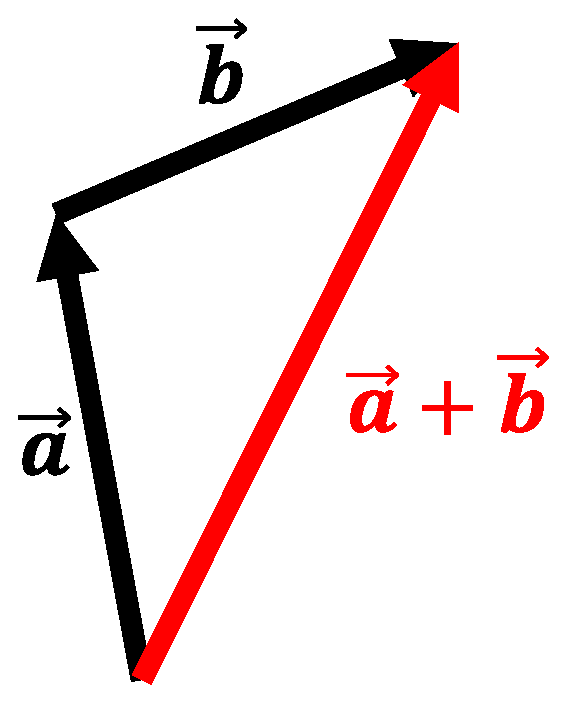
\includegraphics{img/vector_tasizan.eps}
            }
        \end{center}
        \caption{ベクトルの足し算}
        \label{fig:vector_tasizan}
    \end{figure}

    次は引き算だ.これも先と同様に
    \[
    \vec{a}-\vec{b}
    \]
    とすればよいが.これで十分な理解とは言えない.
    \[
    \vec{a}+ (-\vec{b})
    \]
    とすることでマイナスのベクトルを考えてみる.

    負の大きさというのが少しイメージしにくい\footnote{大きさは0以上の値をとる.絶対値の考えを使うからだ.}が結局のところ向きが逆\footnote{ベクトルは向きが存在するので,基本的には存在しない"負の大きさ"というものを考えることができる.向きを逆にするということで対処するのだ.}になる.図\ref{fig:vector_mainasu}のようなことだ.
    \begin{figure}[htbp]
        \begin{center}
            \resizebox{!}{3cm}{
            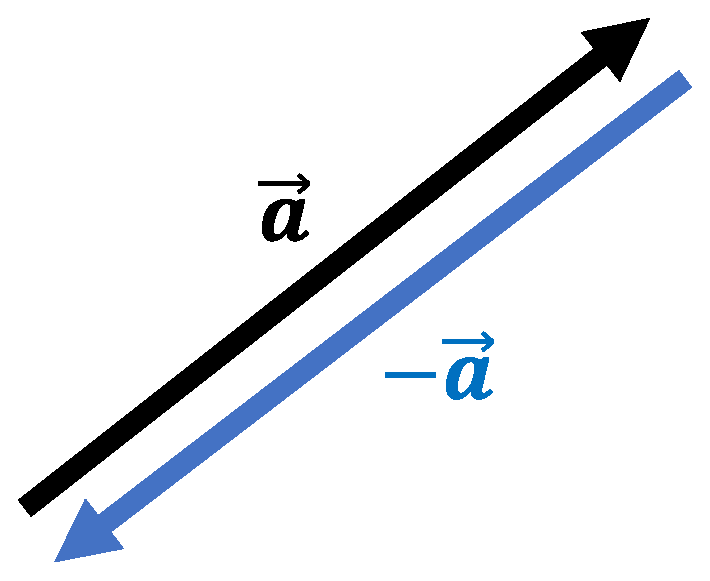
\includegraphics{img/vector_mainasu.eps}
            }
        \end{center}
        \caption{マイナスのベクトル}
        \label{fig:vector_mainasu}
    \end{figure}
    %

    マイナスのベクトルを導入したうえでベクトルの引き算を図示する.図\ref{fig:vector_hikizan1}のようになる.さらにマイナスのベクトルをもとに戻すと図\ref{fig:vector_hikizan2}のようになる.ここからベクトルの引き算は2つのベクトルの終点同士を引くベクトル(ここでは$\vec{b}$)から引かれるベクトル(ここでは$\vec{a}$)へつなげればいいことがわかる.
    %
    \begin{figure}[htbp]
        \begin{center}
            \begin{tabular}{c}

                \begin{minipage}{0.45\hsize}
                    \begin{center}
                        \resizebox{0.7\hsize}{!}{
                        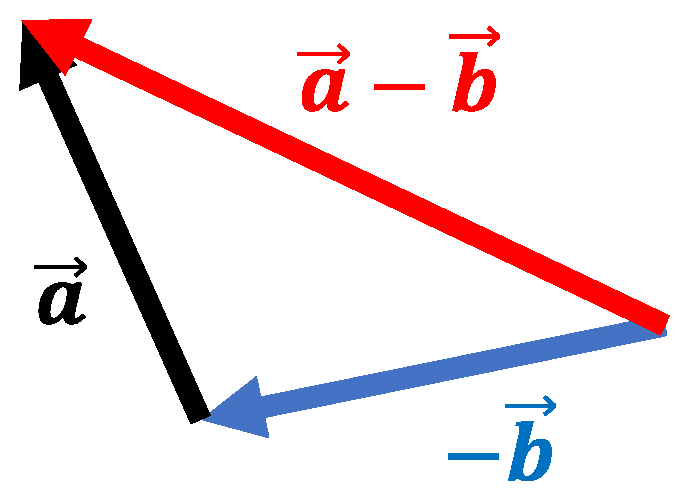
\includegraphics{img/vector_hikizan1.eps}
                        }
                    \end{center}
                    \caption{ベクトルの引き算1}
                    \label{fig:vector_hikizan1}
                \end{minipage}

                \begin{minipage}{0.45\hsize}
                    \begin{center}
                        \resizebox{0.7\hsize}{!}{
                        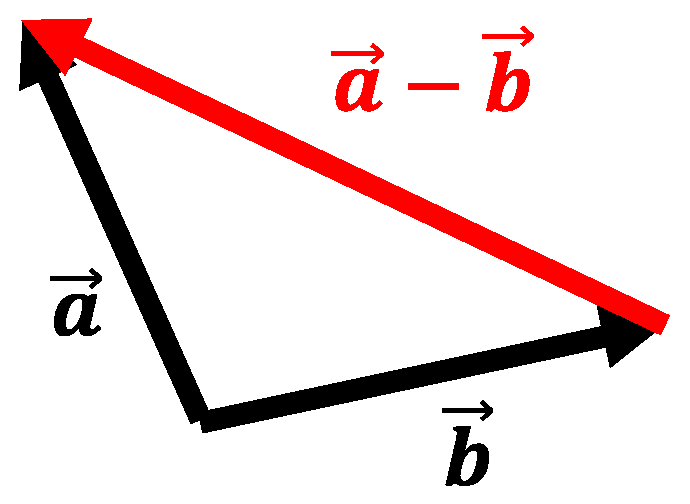
\includegraphics{img/vector_hikizan2.eps}
                        }
                    \end{center}
                    \caption{ベクトルの引き算2}
                    \label{fig:vector_hikizan2}
                \end{minipage}


            \end{tabular}
        \end{center}

    \end{figure}



    \subsection{積算}
    結論からいうとベクトル同士の掛け算はできない.と言ってしまうと残念な話であるが掛け算のような計算を導入することで対処する.

    まずはベクトルと定数の掛け算を考える.ベクトルの定数倍は大きさのみに作用する.$k\vec{a}$は図\ref{fig:vector_tesubai1}のような状態となる.負の数であれば逆向きになることもあわせて理解しよう(図\ref{fig:vector_tesubai2}).
    %

    \begin{figure}[htbp]
        \begin{center}
            \begin{tabular}{c}

                \begin{minipage}{0.45\hsize}
                    \begin{center}
                        \resizebox{!}{3cm}{
                        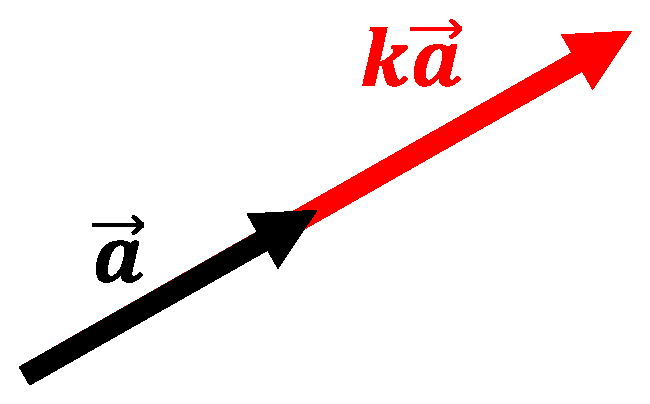
\includegraphics{img/vector_tesubai1.eps}
                        }
                    \end{center}
                    \caption{ベクトルの定数倍1}
                    \label{fig:vector_tesubai1}
                \end{minipage}

                \begin{minipage}{0.45\hsize}
                    \begin{center}
                        \resizebox{!}{3cm}{
                        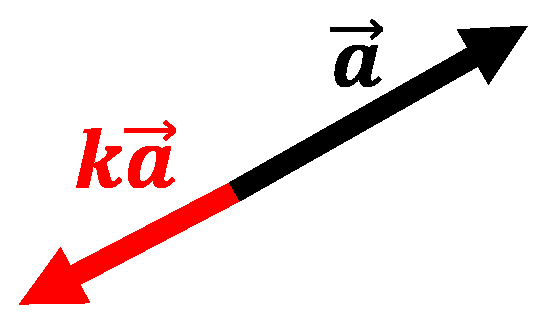
\includegraphics{img/vector_tesubai2.eps}
                        }
                    \end{center}
                    \caption{ベクトルの定数倍2}
                    \label{fig:vector_tesubai2}
                \end{minipage}


            \end{tabular}
        \end{center}

    \end{figure}


    次はベクトル同士の掛け算のような計算,すなわち内積を考える.内積の計算に求められるのは普通の計算で成立する次のような性質だ.
    \begin{enumerate}
        \item 定数倍
        \[
        (ka)\cdot b=k(a\cdot b)
        \]
        \item 交換の法則
        \[
        a\cdot b=b\cdot a
        \]
        \item 分配・結合の法則
        \[
        a\cdot(b+c)=a\cdot b + a\cdot c
        \]
    \end{enumerate}

    これを達成できるように内積を定める.図\ref{fig:vector_naiseki1}のような2つのベクトル$\vec{x},\vec{y}$に対して,
    \begin{equation}
        \vec{x}\cdot\vec{y}=|\vec{x}||\vec{y}|\cos\theta
        \label{eq:def_naiseki}
    \end{equation}
    と内積を定義する.
    %
    \begin{figure}[htbp]
        \begin{center}
            \resizebox{!}{3.5cm}{
            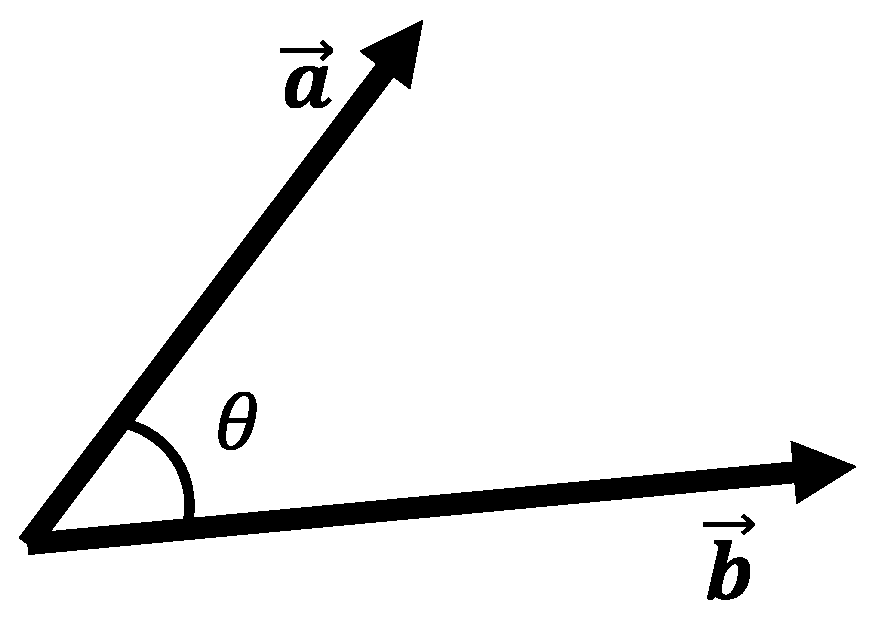
\includegraphics{img/vector_naiseki1.eps}
            }
        \end{center}
        \caption{内積}
        \label{fig:vector_naiseki1}
    \end{figure}

    図形的な理解をすると次のようになる(図\ref{fig:vector_naiseki2}).始点を共有している2つのベクトルにおいて,一方のベクトルの終点から他方のベクトルへ垂線をおろす.垂線の足とベクトルの始点との距離は図においては$|\vec{x}|\cos\theta$となる.これと垂線を下した先のベクトルの大きさ$|\vec{y}|$との積が内積の図形的な理解である.
    %
    \begin{figure}[htbp]
        \begin{center}
            \resizebox{!}{4cm}{
            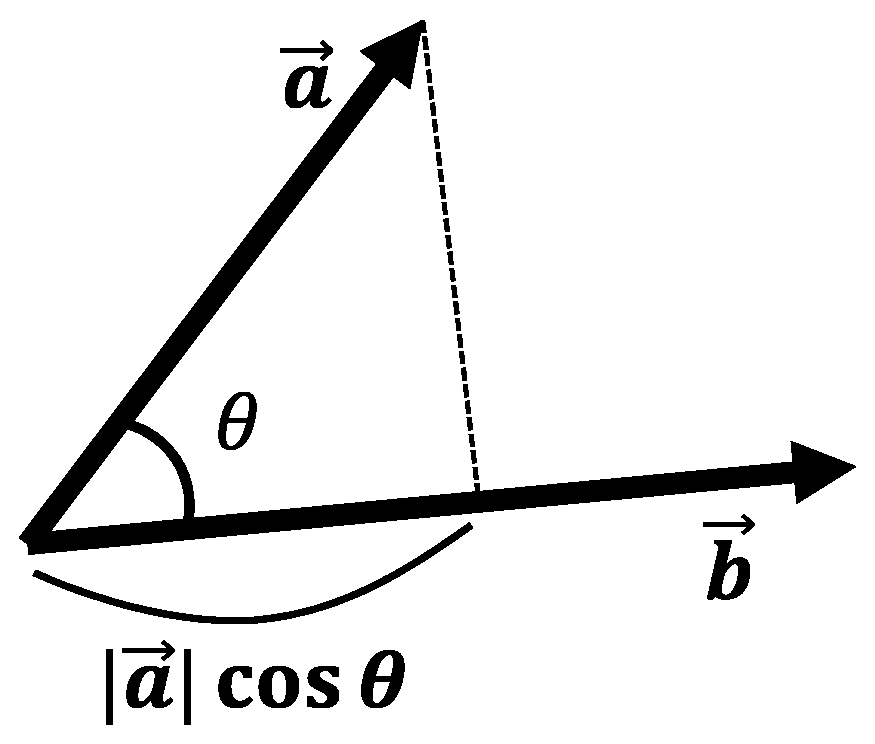
\includegraphics{img/vector_naiseki2.eps}
            }
        \end{center}
        \caption{内積の図形的理解}
        \label{fig:vector_naiseki2}
    \end{figure}




    内積に求められるのは先に挙げた性質と$\vec{x},\vec{y}$の持つ関係だ.$\cos\theta$となっているのは2つのベクトルのなす角が$0\leq\theta\leq\pi$であることからだ.$\sin\theta$では同じ値が2回出てしまう\footnote{$\sin x=\sin (\pi -x)$であることを言っている.}.これで内積は2つのベクトルの大きさと向きの2つの性質を合わせたものになっていることがわかる.

    ここからは内積が先に挙げた3つの性質を満たしているかを確認する内容だ.興味がなければ読み飛ばしてほしい.
    \begin{description}
        \item[定数倍] 定数$c>0$をとる.
        \begin{eqnarray*}
            (c\vec{x})\cdot(\vec{y})&=&|c\vec{x}||\vec{y}|\cos\theta\\
            &=&|c||\vec{x}||\vec{y}|\cos\theta\\
            &=&c(\vec{x}\cdot\vec{y})
        \end{eqnarray*}
        となる.次は$c<0$のとき
        \begin{eqnarray*}
            (c\vec{x})\cdot(\vec{y})&=& \{(-c)(-\vec{x})\}\cdot\vec{y}\\
            &=& |(-c)(-\vec{x})||\vec{y}|\cos(\pi-\theta)\\
            &=&-c|\vec{x}||\vec{y}|(-\cos\theta)\\
            &=&c(\vec{x}\cdot\vec{y})
        \end{eqnarray*}
        となり,定数倍の性質は満たす.図は後半の参考の図\ref{fig:vector_naiseki_tesubai}だ.
        %
        \begin{figure}[htbp]
            \begin{center}
                \resizebox{!}{4cm}{
                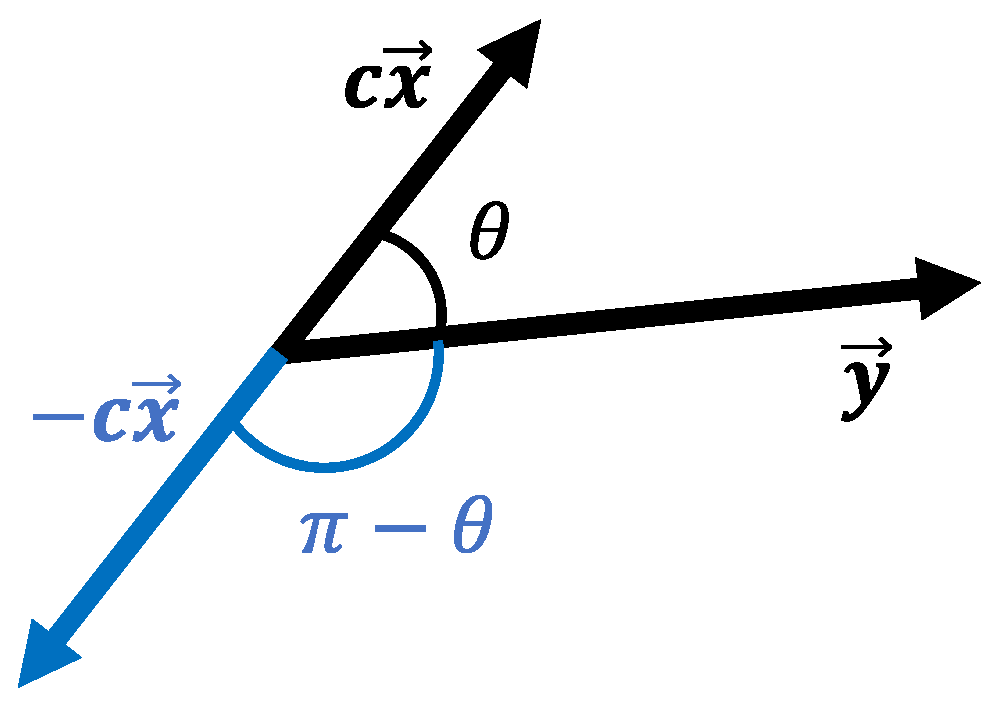
\includegraphics{img/vector_naiseki_tesubai.eps}
                }
            \end{center}
            \caption{内積の定数倍}
            \label{fig:vector_naiseki_tesubai}
        \end{figure}
        \item[交換の法則] 定義の式からも交換が可能であることは明らかだ.
        \[
        \vec{x}\cdot\vec{y}=|\vec{x}||\vec{y}|\cos\theta=|\vec{y}||\vec{x}|\cos\theta=\vec{y}\cdot\vec{x}
        \]
        \item[分配・結合の法則] 図\ref{fig:vector_naiseki_ketugo}の3つのベクトルから$(\vec{x}+\vec{y})\cdot\vec{z}$を考える.
        図\ref{fig:vector_naiseki_ketugo}から
        \[
        |\vec{x}+\vec{y}|\cos\theta= |\vec{x}|\cos\alpha +|\vec{y}|\cos\beta
        \]
        がわかるので,ここから
        \begin{eqnarray*}
            &|\vec{x}+\vec{y}||\vec{z}|\cos\theta= |\vec{x}||\vec{z}|\cos\alpha +|\vec{y}||\vec{z}|\cos\beta &\\
            &\Rightarrow (\vec{x}+\vec{y})\cdot\vec{z} =\vec{x}\cdot\vec{z} + \vec{y}\cdot\vec{z} &
        \end{eqnarray*}
        が計算される.
        %
        \begin{figure}[htbp]
            \begin{center}
                \resizebox{!}{6cm}{
                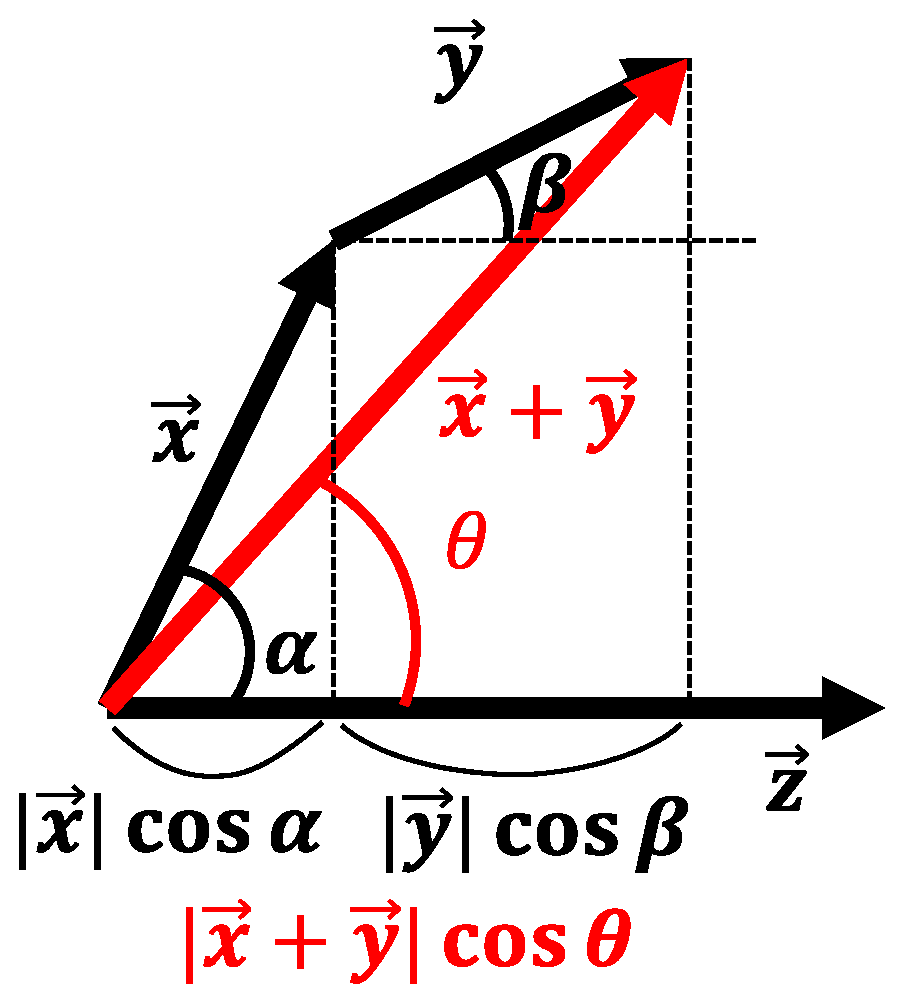
\includegraphics{img/vector_naiseki_ketugo.eps}
                }
            \end{center}
            \caption{結合法則}
            \label{fig:vector_naiseki_ketugo}
        \end{figure}

    \end{description}

    \subsection{2つのベクトルの関係}
    内積の定義式である式(\ref{eq:def_naiseki})から内積$\vec{a}\cdot\vec{b}$に次のことがわかる.
    \begin{eqnarray*}
        \theta =90^\circ=\frac{\pi}{2}&&\\
        &&\Rightarrow \vec{a}\cdot\vec{b} =0\\
        \theta = 0&&\\
        &&\Rightarrow \vec{a}\cdot\vec{b} = |\vec{a}||\vec{b}|
    \end{eqnarray*}
    これは$\cos\theta$の値のうち,特徴的なものから得られる関係だ.ここから次の同値関係がわかる.
    \begin{screen}
        \veczero ではない2つのベクトル\veca ,\vecb において$\vec{a}\cdot\vec{b}=0$であることと$\vec{a}\perp\vec{b}$であることは同値.

        数学的な式に直すと
        \[
        \vec{a},\vec{b}\neq\vec{0},\mmm\vec{a}\cdot\vec{b}=0\mmm\Leftrightarrow\mmm
        \vec{a}\perp\vec{b}
        \]
        と表される.

        この同値関係で重要なのは内積が0であることだけでは,2つのベクトルが垂直なのかがわからないところだ.\veczero であるときも内積は0となることに注意しよう.
    \end{screen}
    \begin{screen}
        \veca を2つで内積をとるとその値は\veca の大きさの2乗となり,${\vec{a}}^2$とは書かない.
        \[
        \vec{a}\cdot\vec{a}=|\vec{a}|^2
        \]
        これは簡単な式で取り上げる必要性もそれほど大きくないかもしれない.しかし,問題を解く上では頻出の関係なのであえて示す.
    \end{screen}

    次に平行な2つのベクトルを考える.これは2つのベクトルのなす角が0または$\pi$であるときだ.このような2つのベクトル\vecx ,\vecy に対しては次の関係が成り立つ.
    \[
    \vec{x}//\vec{y}\mmm \Leftrightarrow\mmm k\vec{x}=\vec{y}\mmm(kは実数)
    \]
    これも当然の式といえる.

    以上の関係は\veca のようなベクトルを利用して計算するときに主に使う式である.それと同時に\veca のようなベクトルは"平行"と"垂直"の2つが関係するときに大きな威力を発揮することを示している.これは逆に平行や垂直といった条件のない問題ではやや計算が困難になるということなので解答の方針を考える際は1つの指標にしてほしい.


    \subsection{$\vec{a}$のようなベクトルの計算のまとめ}
    先までの内容で$\vec{a}$などと表記されるタイプのベクトルを文字式のように計算できることが分かった.足し算や引き算はいつものように計算し,掛け算の部分を$\vec{a}\cdot\vec{b}$のように内積で表現すればいいのだ.

    そして,最初に述べた"向き"は計算できないという問題を\veca のような表現のベクトルでは
    $\vec{a}\cdot\vec{b}$や$|\vec{a}+\vec{b}|^2$といったベクトルをスカラにしてしまう計算によって解決している.




% \end{document}

    \documentclass{jsarticle}
\usepackage[dvipdfmx]{graphics}
\usepackage{amsmath}
\usepackage{amssymb}
\usepackage{ascmac}
\usepackage{bm}
\usepackage{url}
\usepackage{txfonts}

\newcommand{\mmm}{\hspace{3mm}}
\newcommand{\veczero}{$\vec{0}$}
\newcommand{\veca}{$\vec{a}$}
\newcommand{\vecb}{$\vec{b}$}
\newcommand{\veco}{$\vec{o}$}
\newcommand{\vecx}{$\vec{x}$}
\newcommand{\vecy}{$\vec{y}$}
\newcommand{\vecz}{$\vec{z}$}
\newcommand{\mathins}[1]{${#1}$}


\begin{document}
    \section{(1,2)のようなベクトル}
    これは見るからに数字のみの形式をしている.このような表記のベクトルは予めお約束となるベクトルを用意することで向きの計算を回避している.
    \subsection{(1,2)の意味}
    (1,2)のような形をしているベクトルは次のようにあらわすこともできる.
    \[
    (1,2)=\vec{x}+2\vec{y}
    \]
    ここでの$\vec{x}$とはx軸正方向に大きさ1のベクトルを表し,$\vec{y}$はy軸正方向に大きさ1のベクトルを表している.大きさ1のベクトルを特別に単位ベクトルという.この各軸の正方向に向く単位ベクトルをお約束のベクトルとして用意し,その係数だけでベクトルを表すのが(1,2)のようなベクトルの意味だ.

    \subsection{計算}

    前の節の話を持ってくれば$\vec{x},\vec{y}$があれば,あとは係数の計算をするだけで足し算と引き算は計算できる.
    \begin{eqnarray*}
        &&(1,2)+(3,-7)=(1+3,2-7)=(4,-5)\\
        &&(\vec{x}+2\vec{y})+(3\vec{x}-7\vec{y})=4\vec{x}-5\vec{y}
    \end{eqnarray*}

    次は定数倍だ.
    \begin{eqnarray*}
        &&k(1,2)=(k,2k)\\
        &&k(\vec{x}+2\vec{y}) =k\vec{x}+2k\vec{y}
    \end{eqnarray*}
    各成分に定数をかければいい.


    最後は内積だ.だが,その前にお約束のベクトルのみで内積などを計算しておく.
    \[
    \vec{x}\cdot\vec{x}=1,\mmm\vec{y}\cdot\vec{y}=1,\mmm\vec{x}\cdot\vec{y}=0
    \]
    大きさ1であることと,軸は直交していることから計算される.

    これを使って次の内積を計算する\footnote{$(a,b)\cdot(c,d)$という書き方は誤りです.答案には書かないようにしましょう.}.
    \begin{eqnarray*}
        \vec{n}=(a,b),&\mmm&\vec{m}=(c,d)\\
        \vec{n}\cdot\vec{m}&=&(a\vec{x}+b\vec{y})(c\vec{x}+d\vec{y})\\
        &=&ac|\vec{x}|^2 +(ad+bc)\vec{x}\cdot\vec{y}+bd|\vec{y}|^2\\
        &=&ac+bd
    \end{eqnarray*}
    x成分同士,y成分同士の積を足せばよいことがわかる.

    また,複数のベクトルの和としてあらわされているベクトルを掛け算(内積)するときは前もって部分的な内積,大きさの2乗を示す形の書き方をするほうが答案として簡潔でよい.

    \subsection{使用の方針}
    ベクトル入門の章において係数のみによってベクトルを表すタイプを前面に使うことはない.例えば(1,2),(3,4)が与えられていたら,$\vec{a}=(1,2),\vec{b}=(3,4)$として\veca ,\vecb によって計算を進める.そして計算が一段落したら$|\vec{a}|^2=1^2+2^2,|\vec{b}|^2=3^2+4^2,\vec{a}\cdot\vec{b}=3+2\times4$を使う.

    ベクトル入門の章における計算の位置づけは次の図\ref{fig:vector_sanjutukeisan_taikei}のようになっている.

    \begin{figure}[htbp]
        \begin{center}
            \resizebox{!}{6cm}{
            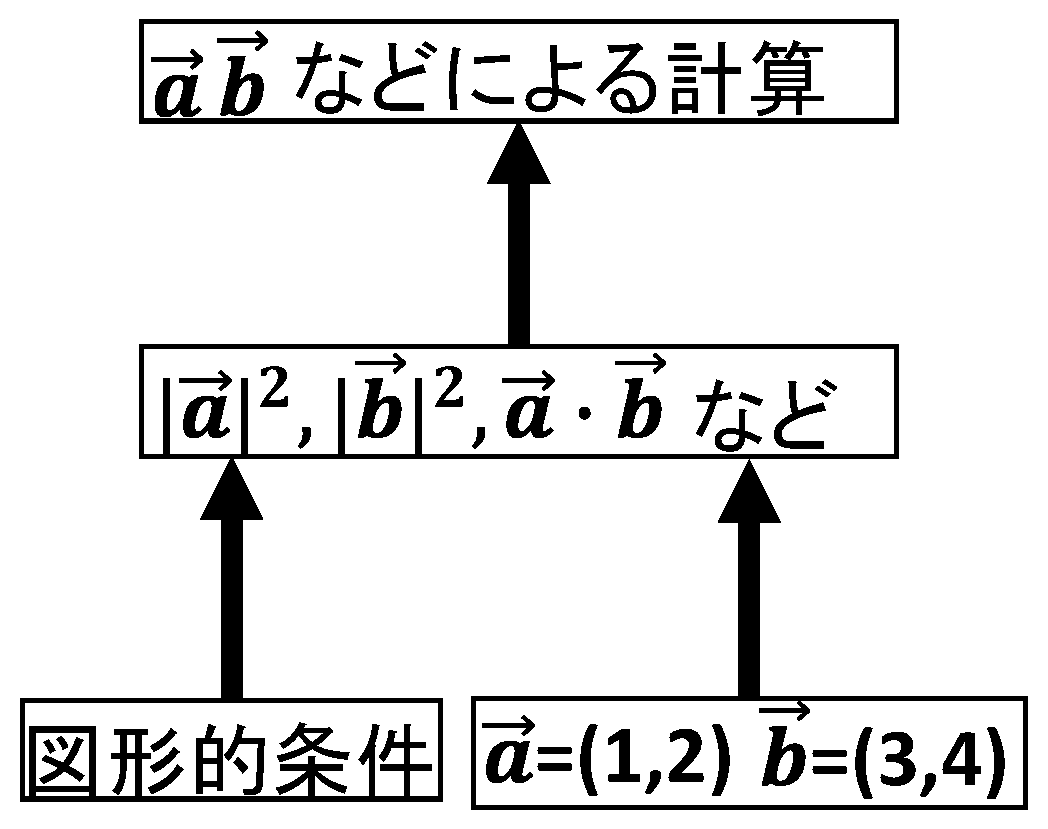
\includegraphics{img/vector_sanjutukeisan_taikei.eps}
            }
        \end{center}
        \caption{ベクトル計算の体系}
        \label{fig:vector_sanjutukeisan_taikei}
    \end{figure}

    したがって,ベクトル入門の章において成分表示で与えられたベクトルは問題の条件と同等の扱いをする.

    \section{ベクトル入門での問題}
    この章の内容で理解できる問題は以下の通りだ.
    \begin{itemize}
        \item 2ベクトルの関係(垂直)
        \item 2ベクトルの関係(平行)
        \item 2ベクトルの関係(角度)
        \item 2点間の距離
        \item ベクトルの成分分解
        \item ベクトルの分解
    \end{itemize}

    以下に問題を示す.解く必要はないので解答を読んでほしい.

    \subsection{2ベクトルの関係(垂直)}
    \begin{itembox}[l]{問題}
        \begin{enumerate}
            \item $\vec{a}=(1,2)$と垂直であり,なおかつ大きさが$2\sqrt{5}$のベクトルを答えよ.
            \item $\vec{b}=(3,0,0)$と垂直なベクトルを2つ挙げよ.ただし,その2つのベクトル同士も垂直であるとする.
        \end{enumerate}
    \end{itembox}

    まずは1番の問題からだ.未知のベクトルを$\vec{x}=(a,b)$とおいて
    \[
    \left\{
    \begin{array}{c}
        a+2b=0\\
        a^2+b^2=20
    \end{array}
    \right.
    \]
    を解けば答えが$(-4,2),(4,-2)$と出る.しかし,これでは芸がない.勘が良いのであれば(1,2)の位置を入れ替え(2,1)とし,どちらかを-1倍することで元のベクトルと垂直なベクトルが得られることがわかるだろう.そうすると,-1倍するのはx成分か,y成分なのかで答えが2つとなることも合点がいく.これを図\ref{fig:vector_90_kaiten}に表してみよう.
    %
    \begin{figure}[htbp]
        \begin{center}
            \resizebox{!}{4cm}{
            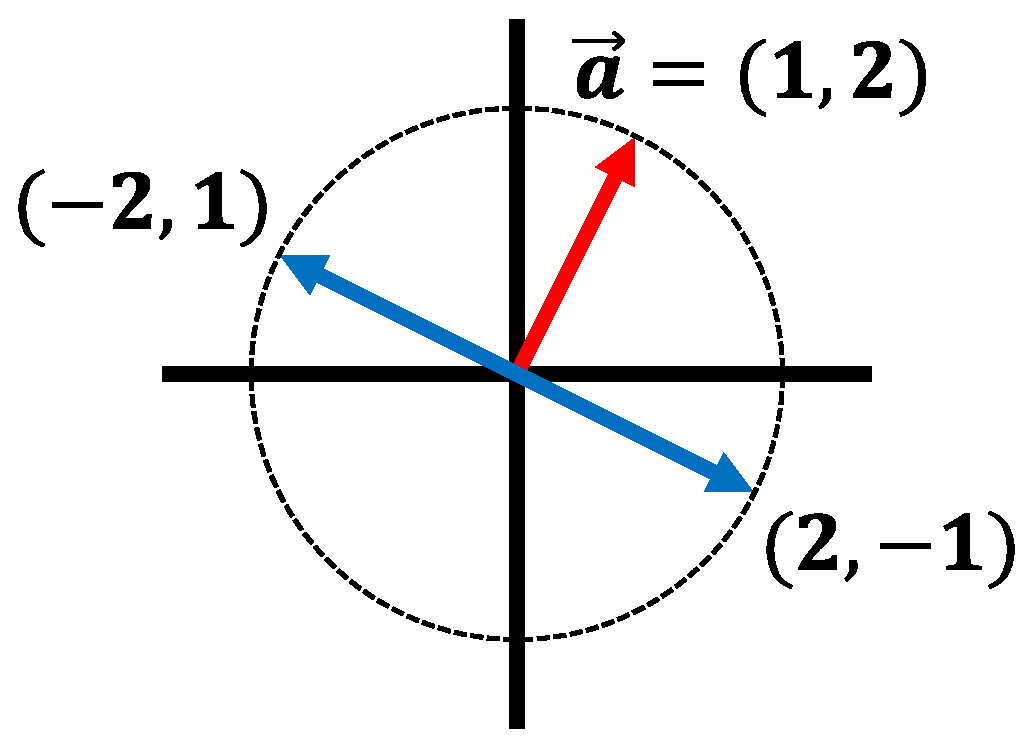
\includegraphics{img/vector_90_kaiten.eps}
            }
        \end{center}
        \caption{ベクトルの回転}
        \label{fig:vector_90_kaiten}
    \end{figure}

    このようにx成分を-1倍すると正の方向に$90^\circ$,y成分を-1倍すると負の方向に$90^\circ$回転することがわかる.これをベクトルの回転\footnote{ベクトルの回転は後の章で扱う.}という.

    回転の発想は法線を扱うときに有効なので頭の隅に置いておきたい.

    2番の問題は3次元ベクトルだ.3つ目の成分はz軸に正方向な単位ベクトルの係数を表している.これは3次元ベクトルの導入に過ぎず,答えの例は(0,1,0),(0,0,1)が挙げられる.3次元ベクトルは計算量こそ多いが2次元ベクトルと同じ話が通用するので拒否反応を起こさないでほしい.

    \subsection{2ベクトルの関係(平行)}
    \begin{itembox}[l]{問題}
        \begin{enumerate}
            \item $\vec{a}=(3,4)$と平行であり,なおかつ大きさが$10$のベクトルを答えよ.
            \item $\vec{b}=(2,5,7)$と平行であり,なおかつ大きさが$19$のベクトルを答えよ.
            \item 四角形ABCDにおいて$\overrightarrow{\mathrm{AB}}=\overrightarrow{\mathrm{DC}}$であるとき,四角形ABCDはどのような四角形であると考えられるか.すべて答えよ.
        \end{enumerate}
    \end{itembox}

    1番の問題は未知のベクトルを$k(3,4)$と置いて次の方程式を解けばよい.
    \[
    25k^2=10^2
    \]
    これより$k=\pm 2$となるので答えは(6,8),(-6,-8)の2つとなる.

    次に2番目の問題だが,これも実数$k$を用意して未知のベクトルを$k(2,5,7)$と置いて計算するのもよいが,この問いではそれが面倒なようにしてある.ここでは単位ベクトルを計算することで答えを求めたい.単位ベクトルは何らかのベクトルを,その大きさで割ることで計算できる.つまり(2,5,7)と同じ向きの単位ベクトルは
    \[
    \frac{1}{\sqrt{2^2+5^2+7^2}}(2,5,7)=\frac{1}{\sqrt{78}}(2,5,7)
    \]
    あとは,大きさが19となるようにすればいいので,答えは
    \[
    \frac{19}{\sqrt{78}}(2,5,7),\mmm \frac{-19}{\sqrt{78}}(2,5,7)
    \]
    の2つとなる.平行なベクトルの計算は単位ベクトルを経由したほうが簡単なことがあるので,発想の引き出しにあるとうれしい.

    最後の問題はベクトルによって平面図形を考える入り口となるような問題だ.問題文より$\overrightarrow{\mathrm{AB}}=\overrightarrow{\mathrm{DC}}$であるがこれは線分$AB$と線分$DC$が大きさが等しく,なおかつ平行であることを示している.これは1組の辺が等しく平行だという平行四辺形の条件を示している.ここから答えは平行四辺形または,ひし形であるとわかる.

    \subsection{2ベクトルの関係(角度)}
    \begin{itembox}[l]{問題}
        \begin{enumerate}
            \item $\vec{a}=(\sqrt{3},1),\vec{b}=(0,2)$のなす角を求めよ.
            \item $\vec{c}=(1,\sqrt{3}),\vec{d}=(t,1)$としたとき,$\vec{c},\vec{d}$が垂直となるときの$t$の値を求めよ.またこのとき,$\vec{d}$がx軸正方向となす角を求めよ.
        \end{enumerate}
    \end{itembox}
    1番の問題は内積の式を変形することで$\cos\theta$を計算することで求められる.\veczero ではない2つのベクトル\veca ,\vecb に対しては次の式が成立する.
    \[
    \cos\theta =\frac{\vec{a}\cdot\vec{b}}{|\vec{a}||\vec{b}|}
    \]
    あとは今回の問題の条件より$\vec{a}\cdot\vec{b}=2,|\vec{a}|=2,|\vec{b}|=2$なので
    \[
    \cos\theta =\frac{1}{2}\mmm \Rightarrow \mmm \theta=60^\circ
    \]

    2番の問題は内積が0という直角の条件から容易に計算できる.
    \[
    t+\sqrt{3}=0\mmm \therefore t=-\sqrt{3}
    \]
    ここから
    \[
    \vec{d}=(-\sqrt{3},1)
    \]
    とわかる.x軸とのなす角は$\tan\theta$を考えるのがよく,求める角度を$\varphi$とすると
    \[
    \tan\varphi = -\frac{1}{\sqrt{3}}\mmm\Rightarrow\mmm\varphi = 150^\circ
    \]
    となる.

    \subsection{2点間の距離}
    \begin{itembox}[l]{問題}
        始点を共有する2つのベクトル\veca ,\vecb は$|\vec{a}|=2,|\vec{b}|=3$,なす角は$\theta=60^\circ$である.このとき2つのベクトルの先端をつないだ線分の長さを求めよ.

        また,この導出にあたり現れる定理は何か.
        %
    \end{itembox}

    ベクトルの先端の長さを考えるとは$|\vec{a}-\vec{b}|$の計算と分かれば話は早い.まずは条件より$\vec{a}\cdot\vec{b}=3$と計算する.あとは大きさの2乗を計算する.
    \begin{eqnarray*}
        |\vec{a}-\vec{b}|^2 &=& |\vec{a}|^2+|\vec{b}|^2-2\vec{a}\cdot\vec{b}\\
        &=&4+9-6=7\\
        \therefore |\vec{a}-\vec{b}|&=&\sqrt{7}
    \end{eqnarray*}

    \begin{figure}[htbp]
    \begin{center}
        \resizebox{!}{3cm}{
        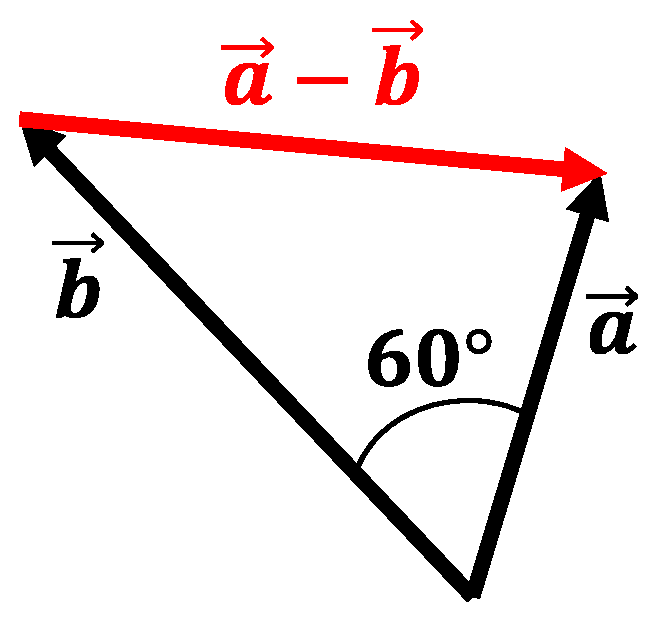
\includegraphics{img/vector_nyumon1.eps}
        }
    \end{center}
    \caption{2点間の距離}
    \label{fig:vector_nyumon1}
    \end{figure}
    ベクトルとスカラを結ぶ方法のおさらいとなる問題だ.そしてこの問題の式を図\ref{fig:vector_nyumon1}とともに見てみる.
    \[
    |\vec{a}-\vec{b}|^2 = |\vec{a}|^2+|\vec{b}|^2-2\vec{a}\cdot\vec{b}
    \]
    をベクトルではない表記に変えてみる.
    \[
    \mathrm{AB}^2 =\mathrm{OA}^2+\mathrm{OB}^2-2 \mathrm{OA}\cdot \mathrm{OB}\cos\theta
    \]
    これは紛れもない余弦定理の公式だ.これはベクトルを利用した余弦定理の証明となっている.


    \subsection{ベクトルの成分分解}
    ベクトルと座標を結びつけるために必要な知識だ.
    \begin{itembox}[l]{問題}
        \begin{enumerate}
            \item 大きさ2,x軸の正方向となす角が$30^\circ$のベクトルのx成分とy成分を答えよ.
            \item 大きさ1,x軸の正方向となす角が$\alpha$となるベクトルを\veca ,大きさ1,x軸の正方向となす角が$\beta$となるベクトルを\vecb とする.$\vec{a}+\vec{b}$のx成分とy成分を2通りの方法で表現せよ.
        \end{enumerate}
    \end{itembox}

    1番の問題は数3における極座標の理解に共通する.答えは$(2\cos30^\circ,2\sin30^\circ)=(1,\sqrt{3})$となる.
    %

    次の問題こそ図がないとわからないだろう.問題の性質上$\alpha<\beta$として問題ない\footnote{2つの単位ベクトルのうち,x軸の正方向となす角が小さいほうを$\alpha$,大きいほうを$\beta$としているに過ぎない.}.
    %
    \begin{figure}[htbp]
        \begin{center}
            \resizebox{!}{5cm}{
            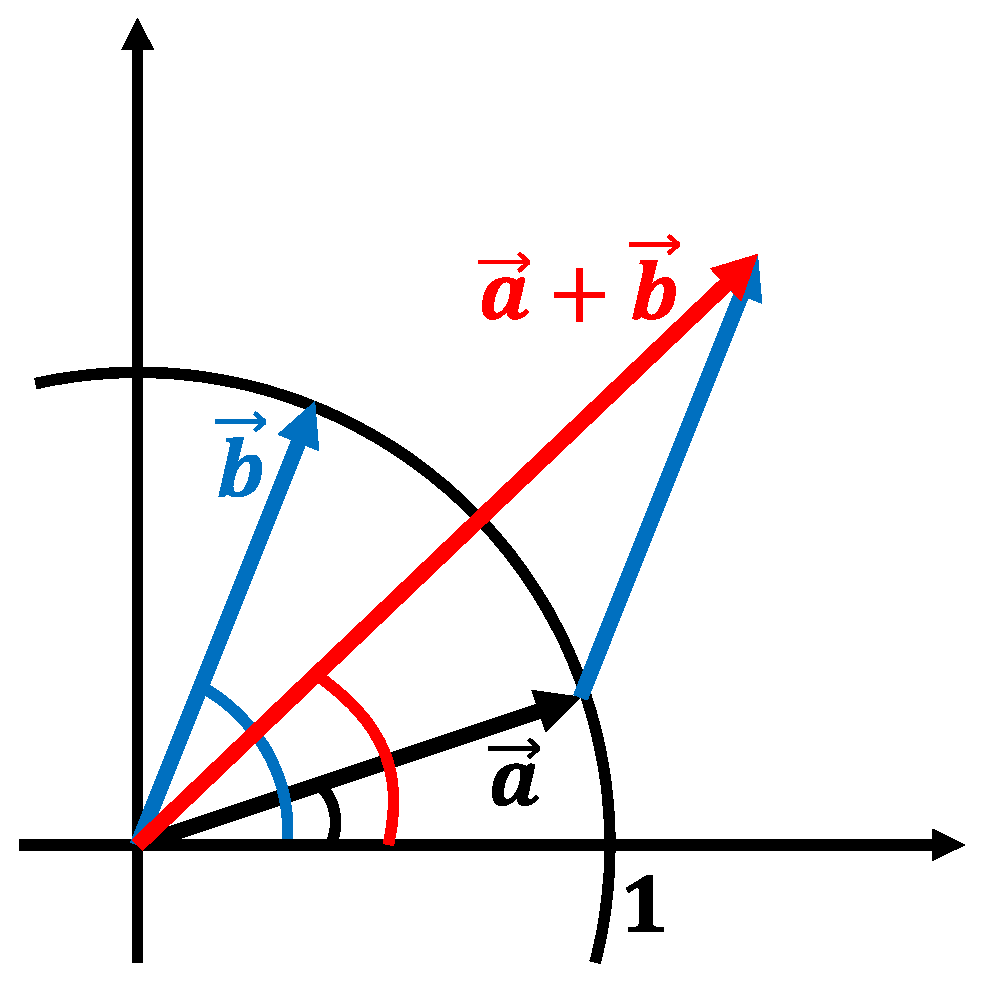
\includegraphics{img/vector_nyumon2.eps}
            }
        \end{center}
        \caption{単位ベクトルの和}
        \label{fig:vector_nyumon2}
    \end{figure}
    まずは1通り目の表現だ.これは単純に成分ごとの計算をすればいい.
    \[
    \vec{a}+\vec{b}=(\cos\alpha+\cos\beta,\mmm\sin\alpha+\sin\beta)
    \]
    次は図\ref{fig:vector_nyumon2}を見てそこから成分表示をする.角度は$\alpha,\beta$の平均をとればいい.あとは$|\vec{a}+\vec{b}|$がわかればいい.これはすでに解いた問題と同じだ.
    \begin{eqnarray*}
        |\vec{a}+\vec{b}|^2&=& |\vec{a}|^2+|\vec{b}|^2 +2\vec{a}\cdot\vec{b}\\
        &=& 2+2\cos(\beta-\alpha)\\
        &=& 2 +2\left(2\cos^2\frac{\beta-\alpha}{2}-1\right)\mmm
        \left(\because \cos\theta=2\cos^2\frac{\theta}{2}-1\right)\\
        &=&4\cos^2\frac{\beta-\alpha}{2}
    \end{eqnarray*}
    さて$\beta-\alpha$はベクトルのなす角であるから$0<|\beta-\alpha|<\pi$である.その半分は$0<|(\beta-\alpha)/2|<\pi/2$と分かる.ここから
    \[
    \cos\frac{\beta-\alpha}{2}=\cos\frac{\alpha-\beta}{2}>0
    \]
    となる.
    \[
    |\vec{a}+\vec{b}|^2=4\cos^2\frac{\beta-\alpha}{2}\mmm \Rightarrow\mmm
    |\vec{a}+\vec{b}|=2\cos\frac{\alpha-\beta}{2}
    \]
    最終的に2つ目の成分表示は
    \[
    \vec{a}+\vec{b}= \left(
    2\cos\frac{\alpha-\beta}{2}\cos\frac{\alpha+\beta}{2},\mmm2\cos\frac{\alpha-\beta}{2}\sin\frac{\alpha+\beta}{2}
    \right)
    \]
    となる.

    問題自体はこれで終わりだが,2番の問題の結果からx,yの成分同士で等式を立てることで次の2式を得ることができる.
    \begin{eqnarray*}
        \cos\alpha+\cos\beta &=&2\cos\frac{\alpha-\beta}{2}\cos\frac{\alpha+\beta}{2}\\
        \sin\alpha+\sin\beta &=&2\cos\frac{\alpha-\beta}{2}\sin\frac{\alpha+\beta}{2}
    \end{eqnarray*}
    これは三角関数の和積の公式だ.ベクトルを用いて三角関数の公式の導出をしたことになる.

    \subsection{ベクトルの分解}
    ベクトルを任意の2つのベクトルの和に分解するという問題だ.これは単に連立方程式の問題となるが色々なところに現れる発想だ.
    \begin{itembox}[l]{問題}
        \begin{enumerate}
            \item ベクトル(1,2)を$\vec{a}=(3,-4),\vec{b}=(-5,7)$を用いた式で表せ.
            \item ベクトル(1,-1)を\mathins{\vec{a}=(3,4),\vec{b}=(4,-3)}を用いた式で表せ.ただし,\mathins{\vec{a}\cdot\vec{b}=0}であることを用いること.
        \end{enumerate}
    \end{itembox}
    1番の問題は\veca ,\vecb の係数を$x,y$とすると
    \[
    (1,2)=x(3,-4)+y(-5,7)
    \]
    という式が立つ.あとは成分ごとに分けて連立方程式とすると$x=17,y=10$を得る.単純な問題である.

    2番の解法が発想として少しだけ大事である.こちらも1番と同様にして連立方程式を立てれば計算はできる.しかし,これでは内積の利用ができない.\mathins{\vec{f}=(1,-1)}として以下のように計算される.
    \begin{align*}
        \vec{f} &= x\vec{a}+y\vec{b}\\
        \vec{f}\cdot\vec{a}&= x\vec{a}\cdot\vec{a} +y\vec{b}\cdot\vec{a}\\
        &= x |\vec{a}|^2 \quad (\because \vec{a}\perp \vec{b})\\
        \therefore x &= \frac{\vec{f}\cdot\vec{a}}{|\vec{a}|^2}\\\\
        \vec{f}\cdot\vec{b}&= x\vec{a}\cdot\vec{b} +y\vec{b}\cdot\vec{b}\\
        &= y|\vec{b}|^2 \quad (\because \vec{a}\perp \vec{b})\\
        \therefore y&=\frac{\vec{f}\cdot\vec{b}}{|\vec{b}|^2}
    \end{align*}

    計算すると\mathins{x=\frac{-1}{25},y=\frac{7}{25}}となる.
    垂直であるという条件はベクトルを扱う上で最も強力な条件の1つである.その恩恵は計り知れないので常にベクトルのなす角には注意が必要だ.




\end{document}



\newpage

    \chapter{ベクトルと図形}
    前章ではベクトルの算術的な計算に注目しベクトルの計算法とスカラ量との結びつけを学習した.
    本章ではベクトルをそのまま扱い平面図形・空間図形などの問題を通してベクトルの有用性を体感したい.
    \documentclass[dvipdfmx]{jsarticle}
\usepackage[dvipdfmx]{graphics}
\usepackage{amsmath}
\usepackage{amssymb}
\usepackage{ascmac}
\usepackage{bm}
\usepackage{url}
\usepackage{txfonts}
\usepackage{tikz}
\newcommand{\mmm}{\hspace{3mm}}
\newcommand{\veczero}{$\vec{0}$}
\newcommand{\veca}{$\vec{a}$}
\newcommand{\vecb}{$\vec{b}$}
\newcommand{\veco}{$\vec{o}$}
\newcommand{\vecx}{$\vec{x}$}
\newcommand{\vecy}{$\vec{y}$}
\newcommand{\vecz}{$\vec{z}$}
\newcommand{\vecrm}[1]{$\overrightarrow{\mathrm{ #1 }}$}
\newcommand{\vecins}[1]{$\vec{#1}$}
\newcommand{\mathins}[1]{${#1}$}

\begin{document}

    \section{図形の中でのベクトル}
    図\ref{fig:vector_tyokuhotai}のような直方体を例に挙げる.直方体の辺をベクトルとしてみると対角線に相当するベクトル\vecrm{OF}は
    \[
    \overrightarrow{\mathrm{OF}}=\overrightarrow{\mathrm{OA}}+
    \overrightarrow{\mathrm{AB}}+\overrightarrow{\mathrm{BF}}
    \]
    など,複数の表現をすることができる.図形の中のベクトルは単純で,見た通りに点を並べてベクトルとしてしまえばよい.
    \begin{figure}[htbp]
        \begin{center}
            \resizebox{!}{5cm}{
            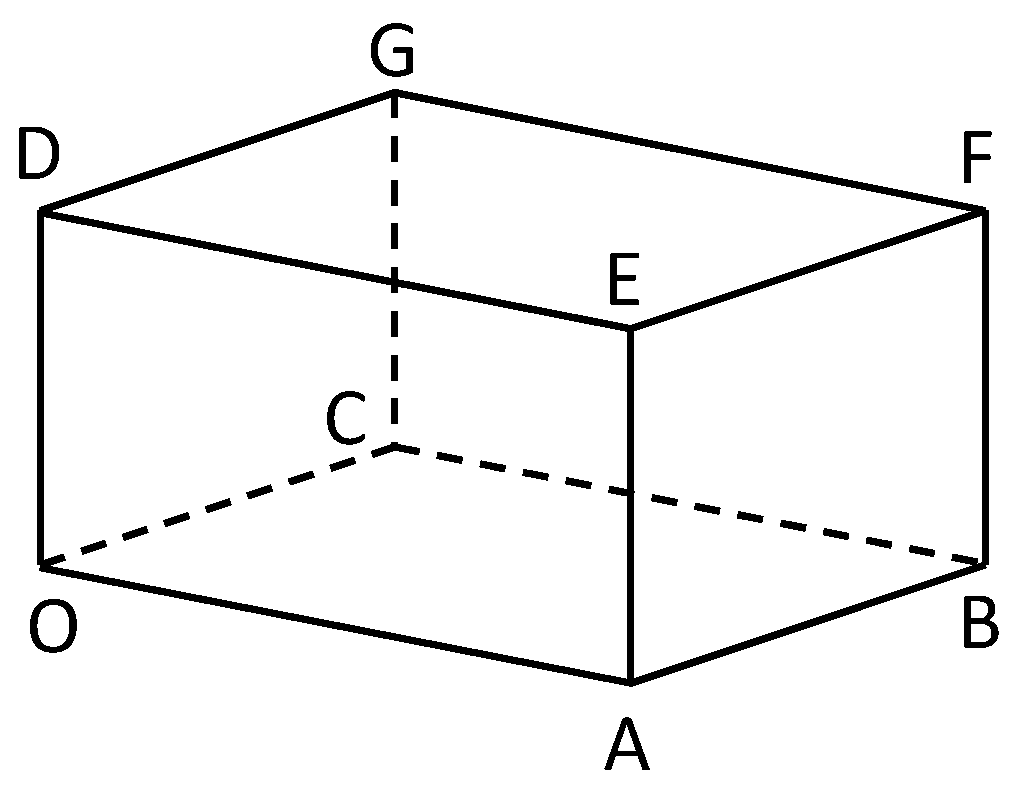
\includegraphics{img/vector_tyokuhotai.eps}
            }
        \end{center}
        \caption{直方体}
        \label{fig:vector_tyokuhotai}
    \end{figure}

    ただ,いちいち始点と終点を明示して表現するタイプのベクトルは書くのが面倒だ.加えて,1つのベクトルに対して複数の表現が存在するのは数学的にあまり好ましくはない.ここで3つのベクトルを代表として次のようにおく.
    \[
    \overrightarrow{\mathrm{OA}}=\vec{a},\mmm\overrightarrow{\mathrm{OC}}=\vec{c},
    \mmm \overrightarrow{\mathrm{OD}}=\vec{d}
    \]
    このようにすると
    \[
    \overrightarrow{\mathrm{OF}}=\vec{a}+\vec{c}+\vec{d}
    \]
    となる.ほかにも点Oからのベクトルに限り,$\vec{a},\vec{c},\vec{d}$を用いて簡潔に表現することができる.図形の中に1つ基準となる点を用意し,そこからの数個のベクトルによって図形上の任意の点を表現する方法はよく使われるので覚えておきたい.

    このような,"定点"を用意してベクトルを簡潔に表す,という発想が位置ベクトルにつながる.


    \section{位置ベクトル}
    算術的な計算のとき,$\vec{a},\vec{b}$はあくまで大きさと向きを備えた記号として扱ってきた.しかし,平面の図形となると始点と終点のほうが際立って扱われる.このことを前提に話を進めよう.

    \subsection{始点と終点\label{sub_sitenshuten}}
    先にも述べたようにベクトル入門におけるベクトルはあくまでベクトル量という意味でしかなかった.しかし,図形の問題におけるベクトルは始点と終点をつないだ有向線分という側面が強く現れる.
    始点と終点という意識が最も顕著に表れるのは$\overrightarrow{\mathrm{AB}},\overrightarrow{\mathrm{CD}}$といった始点と終点をそのまま書いてしまう書き方だ.

    このように図形におけるベクトルは始点と終点の2つで決定される.
    % 計算自体はベクトル入門で扱った方法でよい.

    \subsection{始点の共有\label{sub_sitenkyoyu}}
    直交座標を考えると,その座標というのはすべて原点からとってある.当たり前のことではあるが何か物の位置を定めるには,その基準となる定点が必要になるだろう.これをベクトルで考えてみる.

    図\ref{fig:vector_siten_kyoyu}のように定点Oから各点に有向線分を伸ばす.それらは\vecrm{OA} ,\vecrm{OB} などと表現される.このように必ず始点が一致しているベクトルを考えると,その始点をわざわざ書くことに一体どれほどの意味があるだろうか.これは必要ないと言っていいだろう.

    %
    \begin{figure}[htbp]
        \begin{center}
            \resizebox{!}{4cm}{
            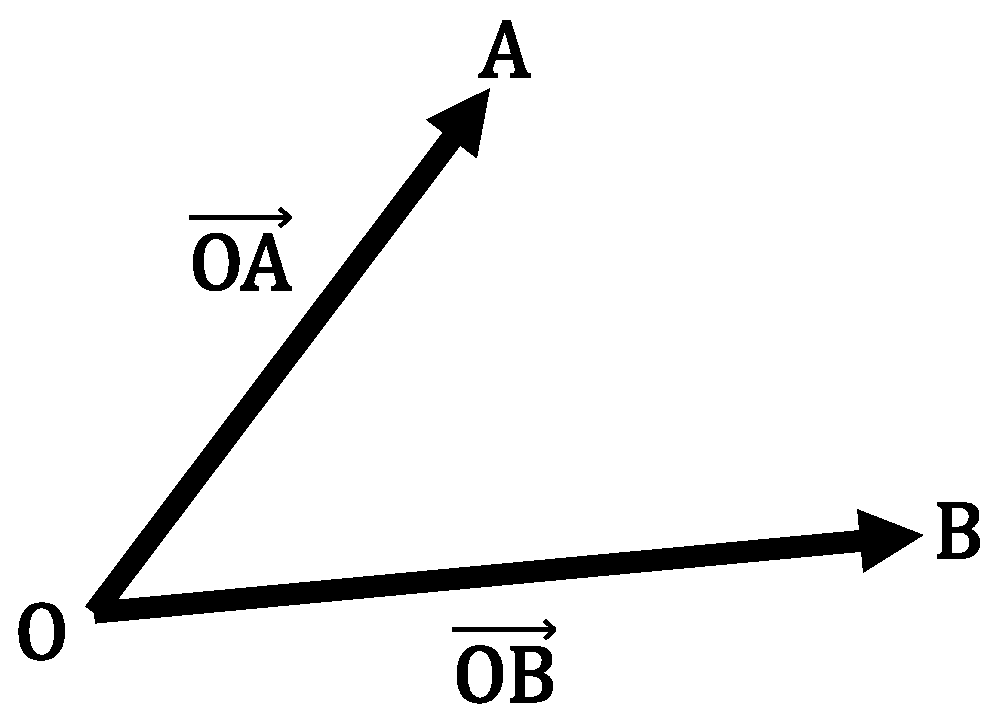
\includegraphics{img/vector_siten_kyoyu.eps}
            }
        \end{center}
        \caption{始点を共有した2ベクトル}
        \label{fig:vector_siten_kyoyu}
    \end{figure}

    このように始点を共有させるという条件のもと,さまざまな点へのベクトルを考えると,
    それは終点のみに注目している状態だということができる.

    \subsection{位置ベクトル}
    図\ref{fig:vector_hukusu_ten}のように空間に点がいくつかある状態を考える.
    %
    \begin{figure}[htbp]
        \begin{center}
            \resizebox{!}{3cm}{
            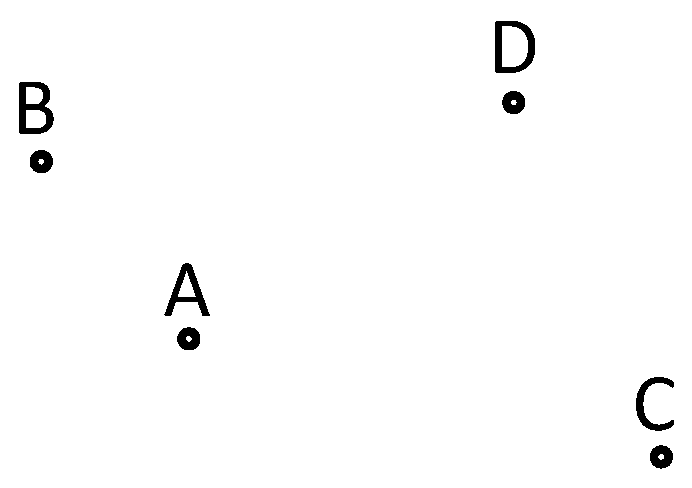
\includegraphics{img/vector_hukusu_ten.eps}
            }
        \end{center}
        \caption{空間上の複数の点}
        \label{fig:vector_hukusu_ten}
    \end{figure}

    このような状態でベクトルを作ると\vecrm{AB} のような2点の位置関係を表すベクトルができ,点Aや点Bだけに注目するようなベクトルは生まれない.
    ここでは\ref{sub_sitenkyoyu}節で扱った始点の共有の考え方を使う.
    % しかし,ここで前の小節で扱った始点の共有の考え方を使う.

    空間の中にどこでもいいから始点となる点Oを用意し,そこから\vecrm{OA} ,\vecrm{OB} などを考えてゆくとそれらのベクトルは終点であるAやBの位置のみを表すベクトルであるということができる.これを位置ベクトルといい,慣習として$\overrightarrow{\mathrm{OA}}=\vec{a}$のように小文字で書く.

    ここで理解を進めるため直交座標と位置ベクトルの対応をまとめる(表\ref{tab:Cartesian_vector}).

    \begin{table}[htbp]
        \caption{直交座標と位置ベクトル}
        \label{tab:Cartesian_vector}
        \begin{center}
            \begin{tabular}{|c|c|c|}\hline
                &直交座標&位置ベクトル\\ \hline
                基準点&原点&任意に定めた点O\\ \hline
                平面での2成分&x,y成分&大きさと向き\\ \hline
                空間での3成分&x,y,z成分&大きさと向き(2つ)\\ \hline
            \end{tabular}
        \end{center}
    \end{table}

    3次元空間で向きを決定するのに2つの成分が必要\footnote{星空を見上げるときに方角と高さの2つを気にすることから体感できるだろう.つまり,3次元空間で方向を決定しようと思うと2つの要素が必要になる.}だ.

    \subsection{位置ベクトルの理解}
    \ref{sub_sitenshuten}節では,図形の問題を扱う上でのベクトルは始点と終点を結ぶ有向線分の側面が大きいと述べた.しかし,表\ref{tab:Cartesian_vector}に示した位置ベクトルの性質は大きさと向きで決定するベクトル入門で大きく扱ったタイプのベクトルだ.これは始点を考えることがなくなったことが理由だ.そして,このことから位置ベクトルを1度導入したら,計算はベクトル入門におけるものをそのまま使えばよいことがわかる.

    また,大きさと向きで決定するタイプのベクトルはその中身\footnote{成分表示したときの内容.}が最後まで分からないことがほとんどだ\footnote{どの方向に向いていて,どれほどの大きさかはわからないまま問題が解けても良い.}.これは当然のことなので抵抗を感じないようにしてほしい.

    \section{位置ベクトルの利用}
    位置ベクトルの基本的な利用法を扱う.
    % 位置ベクトルの基本的な利用法を示す.理解を助けるため1次元座標との対応を考える.

    \subsection{点同士のベクトル}
    2点A(\veca),B(\vecb)を考える.AからBへのベクトルを\vecrm{AB}とする.これを位置ベクトルで表現すると,
    \[
    \overrightarrow{\mathrm{AB}} =\vec{b}-\vec{a}
    \]
   となる.位置ベクトルが始点を共有しているベクトルであることとベクトルの引き算を利用しているのだ.図\ref{fig:vector_iti_tendosi}がその参考になる.
   %
   \begin{figure}[htbp]
       \begin{center}
           \resizebox{!}{3cm}{
           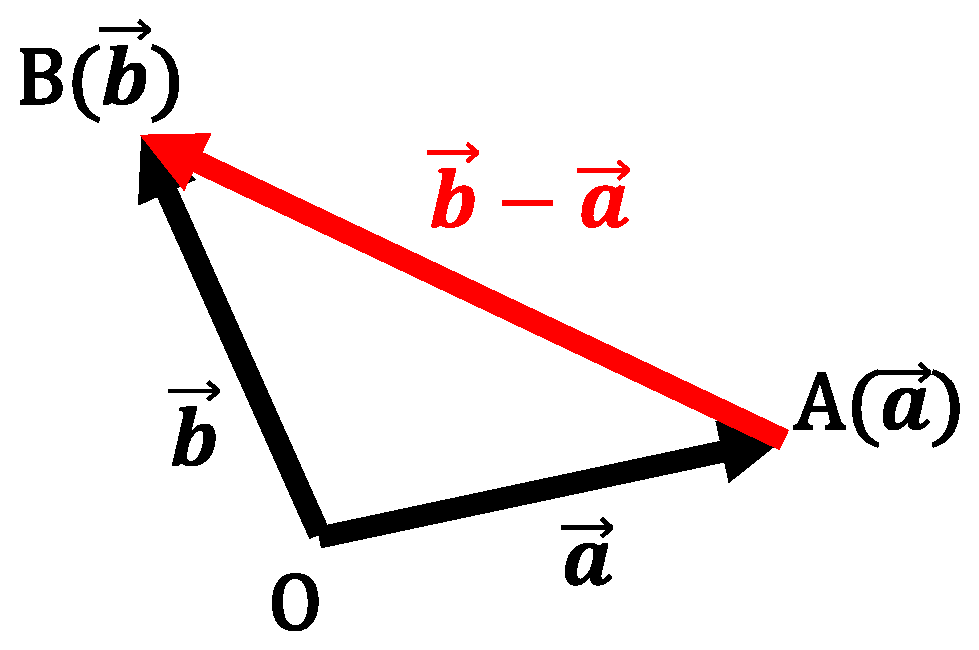
\includegraphics{img/vector_iti_tendosi.eps}
           }
       \end{center}
       \caption{2点間のベクトル}
       \label{fig:vector_iti_tendosi}
   \end{figure}

   \subsection{直線上の点\label{sub_tyokusen_ten}}
   直線AB上の点Pを表したい.例えば点P(\vecins{p})が線分ABをBの方向にABの$l$倍のばした位置にあるとする.直前の内容から$\overrightarrow{\mathrm{AB}} =\vec{b}-\vec{a}$となっていて,条件より
   \[
   \overrightarrow{\mathrm{AP}}=l\overrightarrow{\mathrm{AB}}
   \]
   であることがわかる.あとは位置ベクトルを代入し
   \begin{eqnarray*}
       \vec{p}-\vec{a}&=& l(\vec{b}-\vec{a})\\
       \therefore \vec{p}&=&(1-l)\vec{a}+l\vec{b}
   \end{eqnarray*}
   という結果を得る.係数の和が必ず1となることは頭の隅に置いておこう.


    \subsection{内分点}
    2点A(\veca),B(\vecb)を考える.この2点を$m:n$に内分する点P(\vecins{p})を考える.
    図\ref{fig:vector_iti_naibunten}のような状態だ.
    \vecins{p}は\veca と\vecrm{AB}を$m/(m+n)$倍との和といえよう.
    次のように計算される.

    \begin{eqnarray*}
        \vec{p}&=&\vec{a} +\frac{m}{m+n}\overrightarrow{\mathrm{AB}}\\
        &=& \vec{a}+\frac{m}{m+n}(\vec{b}-\vec{a})\\
        &=& \frac{n\vec{a}+m\vec{b}}{m+n}
    \end{eqnarray*}

    \begin{figure}[htbp]
        \begin{center}
            \resizebox{!}{3cm}{
            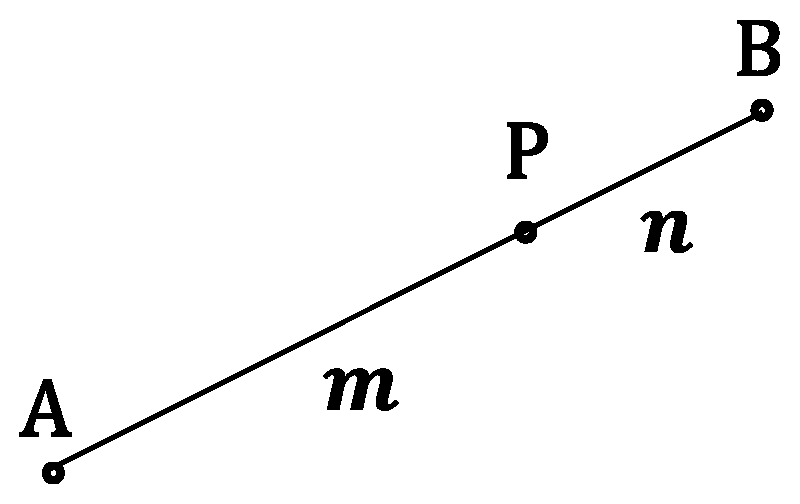
\includegraphics{img/vector_iti_naibunten.eps}
            }
        \end{center}
        \caption{内分点}
        \label{fig:vector_iti_naibunten}
    \end{figure}

    2点A(\veca),B(\vecb)を$m:n$に内分する点P(\vecins{p})が式(\ref{eq:naibunten_kosiki})と表されることを内分点公式という.
    \begin{equation}
        \vec{p}= \frac{n\vec{a}+m\vec{b}}{m+n}
        \label{eq:naibunten_kosiki}
    \end{equation}



    さらに,
    \[
    \frac{n\vec{a}+m\vec{b}}{m+n} =  \frac{n}{m+n}\vec{a} +\frac{m}{m+n}\vec{b}
    \]
    という関係から,係数の和が1となることがすぐにわかる.


    \subsection{外分点}
    2点A(\veca),B(\vecb)を考える.この2点を$m:n$に外分する点Pを考える.$m>n$であれば図\ref{fig:vector_iti_gaibunten1}のように,$m<n$であれば図\ref{fig:vector_iti_gaibunten2}のようになる.
    %
    \begin{figure}[htbp]
        \begin{center}
            \begin{tabular}{c}

                \begin{minipage}{0.45\hsize}
                    \begin{center}
                        \resizebox{!}{3cm}{
                        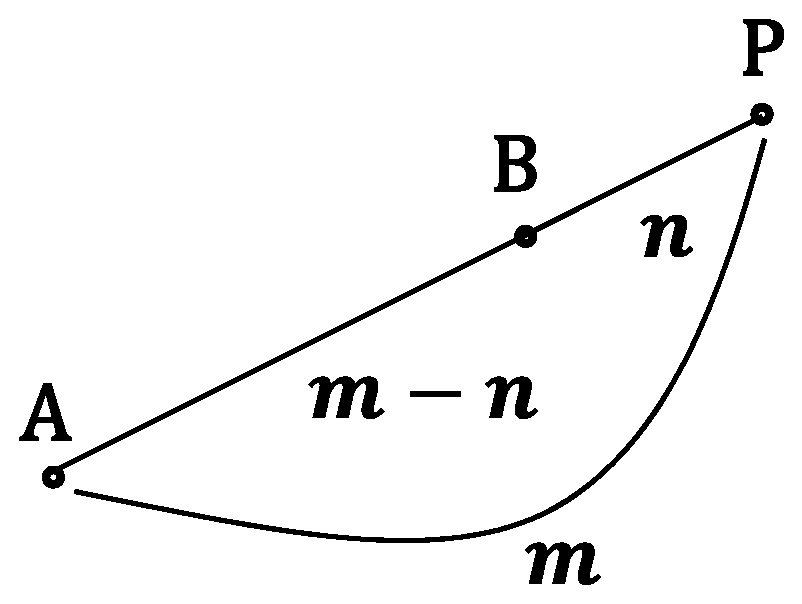
\includegraphics{img/vector_iti_gaibunten1.eps}
                        }
                    \end{center}
                    \caption{\mathins{m>n}}
                    \label{fig:vector_iti_gaibunten1}
                \end{minipage}

                \begin{minipage}{0.45\hsize}
                    \begin{center}
                        \resizebox{!}{3cm}{
                        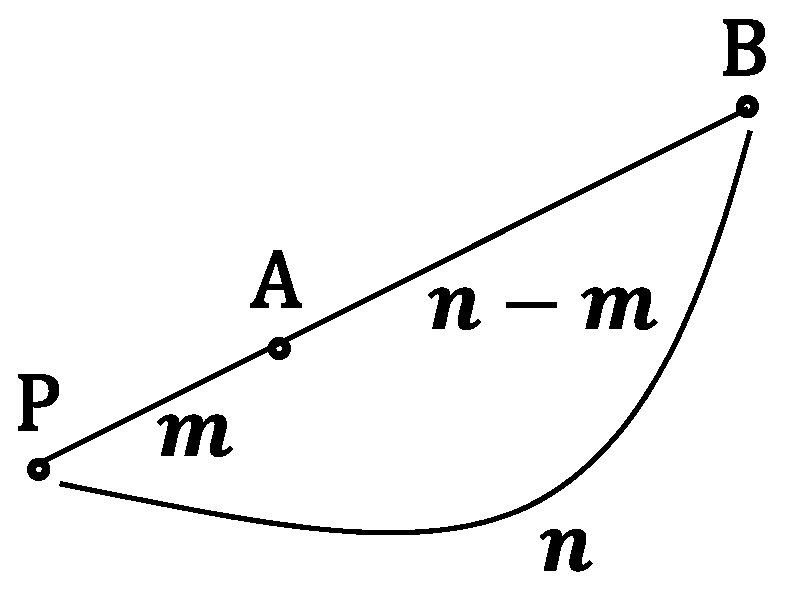
\includegraphics{img/vector_iti_gaibunten2.eps}
                        }
                    \end{center}
                    \caption{\mathins{m<n}}
                    \label{fig:vector_iti_gaibunten2}
                \end{minipage}

            \end{tabular}
        \end{center}
    \end{figure}

    これは$m,n$の大小で場合を分けて考える.$m>n$の場合,AとPに対して内分点公式を使い,Bの位置ベクトルを表す.$\mathrm{AB}:\mathrm{BP}=(m-n):n$より
    \begin{eqnarray*}
        \vec{b} &=& \frac{n\vec{a}+(m-n)\vec{p}}{(m-n)+n}\\
        &=& \frac{n}{m}\vec{a} +\frac{m-n}{m}\vec{p}\\
        \Leftrightarrow \vec{p}&=&\frac{-n\vec{a}+m\vec{b}}{m-n}
    \end{eqnarray*}
    と計算される.

    次に$m<n$の場合,PとBに対して内分点公式を使い,Aの位置ベクトルを表す.$\mathrm{PA}:\mathrm{AB}=m:(n-m)$より
    \begin{eqnarray*}
        \vec{a}&=& \frac{(n-m)\vec{p}+m\vec{b}}{m+(n-m)}\\
        &=& \frac{n-m}{n}\vec{p} +\frac{m}{n}\vec{b}\\
        \Leftrightarrow \vec{p}&=&\frac{n\vec{a}-m\vec{b}}{n-m}\\
        &=&\frac{-n\vec{a}+m\vec{b}}{m-n}
    \end{eqnarray*}
    と計算され,$m,n$の大小関係によらずに同じ結果を得ることができた.

    以上より2点A(\veca),B(\vecb)を$m:n$に外分する点P(\vecins{p})が式(\ref{eq:gaibunten_kosiki})であらわされることを外分点公式という.これはA,Bを$m:(-n)$に内分していると解釈することもできる.
    \begin{equation}
        \vec{p}=\frac{-n\vec{a}+m\vec{b}}{m-n}
        \label{eq:gaibunten_kosiki}
    \end{equation}

    ここでも係数を取り出して考える.
    \[
    \vec{p} = \frac{-n\vec{a}}{m-n}+\frac{m\vec{b}}{m-n}
    \]

    足したら1となるのはここでも同じだ.
    既に\ref{sub_tyokusen_ten}節で一直線上にある点の話でこのことは説明している.
    位置ベクトル\mathins{\vec{a},\vec{b}}を含む直線上の点の位置を2つのベクトルであらわすと係数の和が1となるのだ.ここまでくどいのは問題を解く上で重要な要素となるからである.また,係数がともに正であれば内分点,負のものが含まれれば外分点となることもあわせて覚えよう.

    \subsection{三角形の重心}
    ここまでの位置ベクトルの基本的な利用をおさらいする.


    $\bigtriangleup \mathrm{ABC}$の重心を$\mathrm{G}(\vec{g})$とする.各頂点を$\mathrm{A}(\vec{a}),\mathrm{B}(\vec{b}),\mathrm{C}(\vec{c})$とすると重心の位置ベクトルは
    \[
    \vec{g}=\frac{\vec{a}+\vec{b}+\vec{c}}{3}
    \]
    となる.

    証明の前に,数Aを思い出そう.三角形の重心とは各頂点からの中線の交点と定義されている.さらに,重心は中線を2:1に内分している(図\ref{fig:vector_sankaku_jusin}).

    \begin{figure}[htbp]
        \begin{center}
            \resizebox{!}{3cm}{
            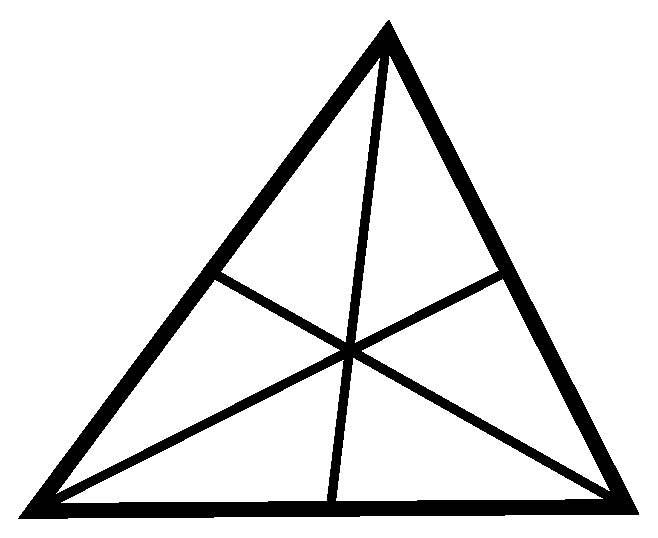
\includegraphics{img/vector_sankaku_jusin.eps}
            }
        \end{center}
        \caption{三角形の重心}
        \label{fig:vector_sankaku_jusin}
    \end{figure}
    %三角形の重心

    では証明に入る.点Aから線分BCの中点へのベクトルを考える.
    \[
    \frac{1}{2}(\vec{b}+\vec{c})-\vec{a}
    \]
    このベクトルを$2/3$倍することで点Aから重心へのベクトルを計算することができる.
    \[
    \overrightarrow{\mathrm{AG}}=-\frac{2}{3}\vec{a}+\frac{1}{3}\vec{b}+\frac{1}{3}\vec{c}
    \]
    となる.最後に$\overrightarrow{\mathrm{AG}}=\vec{g}-\vec{a}$を代入して式を変形することで
    \[
    \vec{g}=\frac{\vec{a}+\vec{b}+\vec{c}}{3}
    \]
    を得る.



    \section{平面図形とベクトル}
    基本的な使い方に加え,より実践的なベクトルの利用を平面図形において扱う.漠然とした話のみをする.具体的には問題を解く際に扱う.そのため読み飛ばしてもらって構わない.



    \subsection{一直線上にある3点(1)}
    点A,B,Cが一直線上にあるとはどういうことか.ベクトル入門の内容から考えるに
    \[
    \overrightarrow{\mathrm{AB}}=k\overrightarrow{\mathrm{AC}}
    \]
    を満たす実数$k$が存在することを証明すればよいだろう.\\

    ここで話はそれるが,高校数学において存在を証明する手段と証明できるものを挙げる.
    \begin{description}
        \item[2次方程式の判別式] 2次方程式に実数の解が存在するのか.また,いくつ存在するのかを明らかにする.
        \item[中間値の定理] 連続な関数であれば,端点の値の間にある値は必ず存在することを証明する.
        \item[平均値の定理] 連続な関数であれば,端の2点で計算される傾きと同じ傾きになる点が少なくとも1つ存在することを証明する.
    \end{description}
    このように高校数学では"存在の証明"の方法が3つしかない.そのほかにも存在だけを考えればよいことは少なくないが,存在だけの言及はできなものと考えたほうが良い.

    では,3点が一直線上にあることを示す$k$の存在はどのように証明するのか.これに対する答えは,$k$の値を明らかにすることだ.値を持つということが存在することの十分条件となる.高度な問題に関しては値を計算すればよいところを,"存在を証明せよ"とわざと誤導することがある.先に挙げた3つの存在証明の性質を理解した上で,場合によっては値を求めることで存在を証明しよう.

    \subsection{一直線上にある3点(2)}
    一直線上にある3点という話を位置ベクトルにも近い話でもう一度扱う.
    図のように定点Oからのベクトル\mathins{\overrightarrow{OA},\overrightarrow{OB}}をとる.これらは一次独立とし,その直線上に点Pがあるとする.
    \begin{figure}[htbp]\centering
        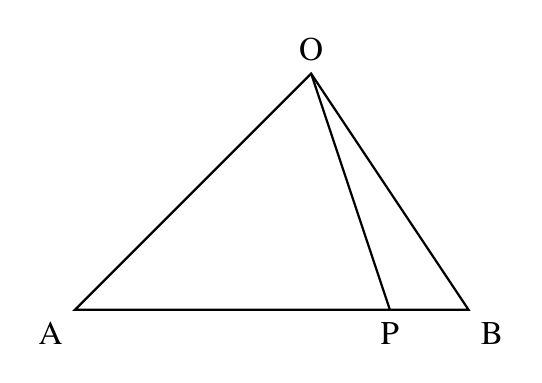
\begin{tikzpicture}\large
            \coordinate (o) at (0,0);
            \coordinate (a) at (-3,-3);
            \coordinate (b) at (2,-3);
            \draw[thick](o)node[above]{O}--(a)node[below left]{A}--(b)node[below right]{B}--cycle;

            \coordinate (p) at (1,-3);
            \draw[thick](o)--(p)node[below]{P};

        \end{tikzpicture}
        \caption{一直線上にある定点}
        \label{tikz:ittyokusen_teiten}
    \end{figure}

    このようにすると,先の話を利用することで
    \[
    \overrightarrow{AB} =k \overrightarrow{AP}\quad{k:\text{実数}}
    \]
    と分かる.これを定点Oからの位置ベクトルとする.
    \begin{align*}
        \overrightarrow{AB} &=k \overrightarrow{AP}\\
        \Leftrightarrow (\overrightarrow{OB}-\overrightarrow{OA})
        &= k(\overrightarrow{OP}-\overrightarrow{OA})\\
        \therefore \overrightarrow{OP}
        &= (1-k)\overrightarrow{OA}+k\overrightarrow{OB}
    \end{align*}

    これは点Pが線分ABを\mathins{k:1-k}に内分したときの内分点公式の結果にも見える.しかし,大事なのは\mathins{k}が実数であるところだ.そのため\mathins{k}は様々な値をとる.例えば\mathins{k}が負の値であるときは点Pは点Aより左側にあり,\mathins{k}が1より大きな値では点Pは点Bの右側にある.つまり,\mathins{k}の値によってPは直線AB上のいかなる点も取ることができる.

    無数のPの位置に対して共通するのは\mathins{\overrightarrow{OA},\overrightarrow{OB}}の係数の値が常に1で一定である点だ.これは逆も成立する話で次のようにまとめられる.
    \begin{itembox}[l]{一直線上の3点の位置ベクトル}
        一次独立なベクトル\mathins{\overrightarrow{OA},\overrightarrow{OB}}に対し,\mathins{\overrightarrow{OP}}が次のように表現されることと,A,B,Pが同一直線上にあることは同値である.
        \[
        \overrightarrow{OP}=s\overrightarrow{OA}+t\overrightarrow{OB},\qquad s+t=1
        \]
    \end{itembox}

    これは定点Oを省略して位置ベクトルでも同様のことが言える.3点が同一直線上にあるということは2つの表現の方法がある.



    \subsection{1次独立}
    この語句は印象に残りやすいものなので,その意味を含めてすでに理解しているかもしれない.空間図形の節でも扱うので読み飛ばしてもらって構わない.

    まずは1次独立とはどういうものなのかを示す.
    \begin{screen}
        ある平面上に存在する\vecins{0} ではない2つのベクトル\veca ,\vecb があるとき,この2つのベクトルが平行でないならば,これらは1次独立であるという.

        さらに,ある平面上で1次独立な関係である2つのベクトル\vecx ,\vecy をとったならば,その平面上の任意のベクトル\vecz は,ある実数$a,b$をもって
        \[
        \vec{z}=a\vec{x}+b\vec{y}
        \]
        と表される.そしてこの実数の組$(a,b)$は,ただ1つに定まる.
    \end{screen}
    これはベクトル入門で扱ったベクトルの分解に関係する話だ.ベクトル入門では分解する先の2つのベクトルはすでに与えられていた.その2つのベクトルとはこの1次独立の関係であるものが選ばれているのだ.

    1次独立で最も重要なのはベクトルを分解した後の係数の組\mathins{a,b} がただ1つに定まるということだ.これを一意性といって,問題を解く上で極めて強力な条件を与える.具体的な使い方は問題で扱う.

    \subsection{斜交座標}
    直交座標というのはベクトルから理解すると,(1,0),(0,1)の2つの単位ベクトルの線形和\footnote{実数をかけた上で,和をとることを線形和という.}によって位置を決定している座標ということになる.
    \[
    (3,-4)=3(1,0)-4(0,1)
    \]
    これは,2つの単位ベクトルが1次独立の関係にあることが重要だ.このため,どのような座標上の点も表すことができる.

    先の小節では平面における1次独立を扱った.1次独立には単位ベクトルである必要も直交している必要もない.つまり,図\ref{fig:vector_shako_zahyo}のような軸をとっても平面上のすべての点を表すことができるのだ.これを斜交座標という.
    %斜交座標の図
    \begin{figure}[htbp]
        \begin{center}
            \resizebox{!}{5cm}{
            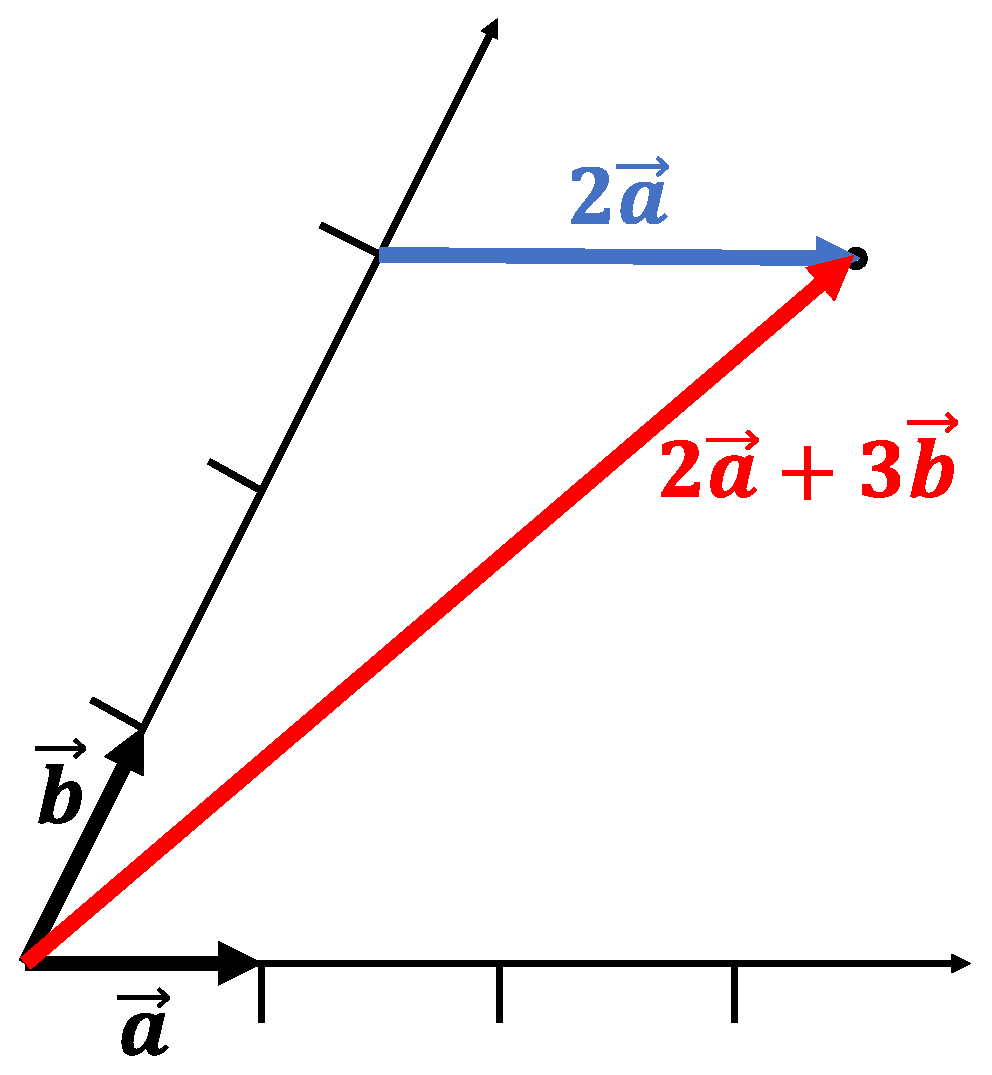
\includegraphics{img/vector_shako_zahyo.eps}
            }
        \end{center}
        \caption{斜交座標}
        \label{fig:vector_shako_zahyo}
    \end{figure}

    図\ref{fig:vector_shako_zahyo}の例では斜交座標における座標は(2,3)となる.

    ベクトル入門では\mathins{(1,2)}のようなベクトルはお約束となるベクトルの係数をとってきた表現であると説明した.斜交座標ではこのお約束のベクトルが1次独立なベクトルの組に置き換わっているのだ.具体的な用法はのちの問題で扱う.



    \section{空間図形とベクトル}

    \subsection{ベクトルの利用価値}
    空間図形に対してベクトルを利用する前に,ベクトルの利用価値について述べたい.ベクトルの本質とは"大きさ"と"向き"を矢印のついた記号に押し込んでしまえば,ベクトル入門で扱った計算法を守るだけで正しい議論が可能であるという点だ.そして,この性質は空間図形において顕著に表れる.位置ベクトルの節において,表\ref{tab:Cartesian_vector}を示した.ここには3次元空間での向きは2つの成分で決定する旨を説明している.つまり,3次元空間を扱うならば本来3つの成分\footnote{大きさ,向き1,向き2の3つ.}を相手にする必要があるのだ.しかし,ベクトルを導入するとその成分は"大きさ","向き"と縮小される.さらに,ベクトル入門の計算則を守れば,矢印のついた記号1つを相手にすればよいことになる.

    これは,ベクトルのルールを守ることを前提に次元数を小さくしているということだ.もちろんベクトルが万能というわけでもない.ベクトルの計算体系は図\ref{fig:vector_sanjutukeisan_taikei}に示した通りであるので,図形的な条件や仮定がない場合は計算自体ができないことも考えれる.2次試験で解法をベクトルに求めるときには注意が必要だ.

    \subsection{一直線上にある3点}
    これは平面での話と同じだ.ただ,問題として出題されるのは空間図形での話が多い.


    \subsection{同じ平面上にあるベクトル}
    3次元空間で1つの平面を決定するときは条件のいずれか1つを満たすことが必要だ.
    \begin{itemize}
        \item 3つの定点がある
        \item 1本の直線と1つの定点がある
        \item 平行な2直線がある
    \end{itemize}
    このような条件に該当するとき平面は決定する.では,始点を共有する2つ異なるのベクトル\veca ,\vecb を考える.ただし,これらはともに\vecins{0} ではない.共有された始点1つと異なる終点2つの3点によって平面が決定する(図\ref{fig:vector_hemen_itijidokusitu}).この2つのベクトルは1次独立な関係になっている.
    %平面とベクトル
    \begin{figure}[htbp]
        \begin{center}
            \resizebox{!}{3cm}{
            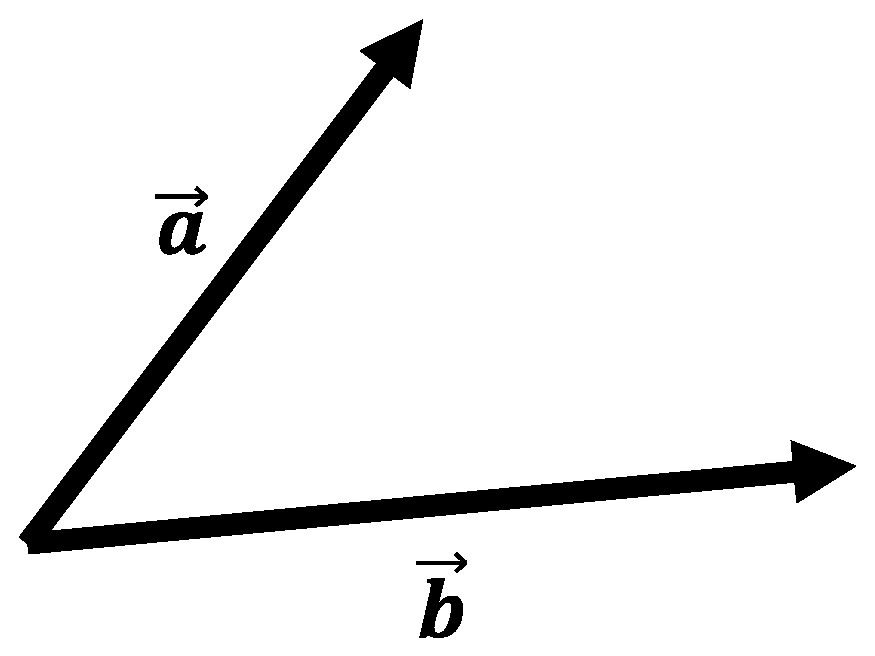
\includegraphics{img/vector_hemen_itijidokusitu.eps}
            }
        \end{center}
        \caption{1次独立}
        \label{fig:vector_hemen_itijidokusitu}
    \end{figure}

    1次独立なベクトル\veca ,\vecb で決定された平面上にベクトル\vecins{c} をとると,いかなる\vecins{c} に対しても
    \[
    \vec{c}=s\vec{a}+t\vec{b}
    \]
    を満たす実数の組$s,t$が存在し,その組はただ1つに定まる.

    あるベクトル\vecins{d} が
    \[
    \vec{d}=k\vec{a}+l\vec{b}\mmm (k,l\in \mathbb{R})
    \]
    であるならば,\vecins{d}は\veca,\vecb の決定する平面上に存在する.

    これは,平面図形での話の続きになる内容だ.結論としては,平面を決定することができる2つのベクトル\footnote{大きさが0ではない,異なる2つのベクトル.}の線形和であらわされるベクトルは,元の2つのベクトルで決定される平面上のベクトルであるといことだ.

    4点が同じ平面に存在するかどうかは,4つのうちの1つを始点とした3つのベクトルで上の関係が成立するのかを確認すればいい.


    \subsection{空間での1次独立}
    3次元空間での1次独立は平面のものとは少し異なる.
    \begin{screen}
        空間に\veczero ではない3つのベクトル\veca,\vecb,\vecins{c} をとる.\veca,\vecb が平行ではなく,
        \[
        \vec{c}=s\vec{a}+t\vec{b}
        \]
        を満たす実数の組\mathins{s,t}がないとき,これらのベクトルは1次独立であるという.

        空間上に1次独立なベクトル\veca,\vecb,\vecins{c} をとる.すると,空間上に存在するすべてのベクトル\vecins{p} は
        \[
        \vec{p}=s\vec{a}+t\vec{b}+u\vec{c}\mmm(s,t,u\in \mathbb{R})
        \]
        と表される.そして実数係数の組\mathins{(s,t,u)}は一意に定まる.
    \end{screen}
    かみ砕いて説明すると,空間における1次独立とは同じ平面に存在しない4つの点の関係を述べている.3点で1つの平面が決定するが,4つ目の点はその平面に存在していない.これは図\ref{fig:vector_tyokuhotai}における\veca,\vecins{c},\vecins{d} の関係だ.


    % \section{ベクトルと図形での問題}
    % \subsection{図形の性質をベクトルから確認}
    % \begin{itembox}[l]{問題}
    %     \begin{enumerate}
    %         \item 平行四辺形
    %         \item
    %         \item
    %         \item
    %         \item
    %         \item
    %         \item
    %     \end{enumerate}
    % \end{itembox}




\end{document}

    \documentclass[dvipdfmx]{jsarticle}
\usepackage{graphics}
\usepackage{amsmath}
\usepackage{amssymb}
\usepackage{amsthm}
\usepackage{mathtools}
\usepackage{ascmac}
\usepackage{bm}
\usepackage{url}
\usepackage{txfonts}
\usepackage{tikz}
% \usepackage{docmute}    %パッケージのダウンロードが必要
\usepackage{tikz}
\usetikzlibrary{calc}
\usetikzlibrary{intersections}



% \usepackage[dvipdfmx]{hyperref}
% \usepackage{pxjahyper}

\newcommand{\mmm}{\hspace{3mm}}
\newcommand{\veczero}{$\vec{0}$}
\newcommand{\veca}{$\vec{a}$}
\newcommand{\vecb}{$\vec{b}$}
\newcommand{\veco}{$\vec{o}$}
\newcommand{\vecx}{$\vec{x}$}
\newcommand{\vecy}{$\vec{y}$}
\newcommand{\vecz}{$\vec{z}$}
\newcommand{\vecrm}[1]{$\overrightarrow{\mathrm{ #1 }}$}
\newcommand{\vecins}[1]{$\vec{#1}$}
\newcommand{\mathins}[1]{${#1}$}


\begin{document}
    \section{ベクトルと図形での問題}
    この章で理解できる問題は以下の通りだ.
    \begin{itemize}
        \item 点の位置関係(同一直線上)
        \item 点の位置関係(同一平面上)
        \item チェバの定理・メネラウスの定理
        % \item 三角形の五心(外心,内心,重心)
        % \item 点,直線,平面の表現
        \item 図形の性質のベクトルによる確認
    \end{itemize}

    \subsection{点の位置関係(同一直線上)}
    \begin{itembox}[l]{問題}
        以下の平行六面体\footnote{向かい合った面が合同な平行四辺形となってる立体を平行六面体という.平行六面体では向かい合った面が平行となる.}において,\mathins{\bigtriangleup\mathrm{ABC}}の重心を\mathins{\mathrm{G}},\mathins{\bigtriangleup\mathrm{PQR}}の重心を\mathins{\mathrm{G}'}とする.このとき,3点\mathins{\mathrm{O},\mathrm{G},\mathrm{G}'}が一直線上にあることを証明せよ.
        %立方体の図

        \begin{centering}
            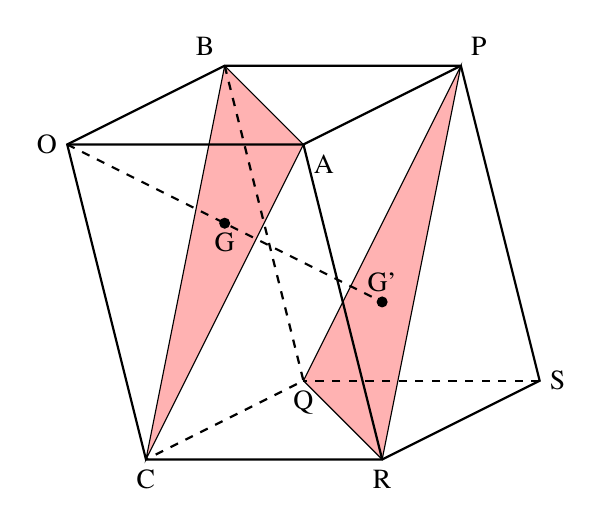
\begin{tikzpicture}
                \coordinate (o) at (0,0);
                \coordinate (a) at (3,0);
                \coordinate (b) at (2,1);
                \coordinate (p) at (5,1);
                \coordinate (c) at (1,-4);
                \coordinate (r) at (4,-4);
                \coordinate (q) at (3,-3);
                \coordinate (s) at (6,-3);

                \filldraw[fill=red!30,draw=black](b)--(a)--(c)--cycle;
                \filldraw[fill=red!30,draw=black](p)--(q)--(r)--cycle;

                \coordinate (g1) at ($0.3333*(a)+0.3333*(b)+0.3333*(c)$);
                \coordinate (g2) at ($0.3333*(p)+0.3333*(q)+0.3333*(r)$);
                \fill (g1)node[below]{G}  circle (2pt);
                \fill (g2)node[above]{G'} circle  (2pt);
                \draw[thick,dashed](o)--(g1)--(g2);

                % 平行六面体の線
                \draw[thick](o)node[left]{O}--(b)node[above left]{B}--(p)node[above right]{P}--(s)node[right]{S}--(r)node[below]{R}--(c)node[below]{C}--cycle;
                \draw[thick](o)--(a)node[below right]{A}--(p);
                \draw[thick](a)--(r);
                \draw[thick,dashed](b)--(q)node[below]{Q}--(c);
                \draw[thick,dashed](s)--(q);

            \end{tikzpicture}
            % \figcaption{立体\label{tikz_question_2_1_ritai}}


        \end{centering}
    \end{itembox}

    Oの基準とする位置ベクトルを置くことで計算を簡単にする.位置ベクトルを次のようにおく.
    \[
    \mathrm{A}(\vec{a}),\mmm\mathrm{B}(\vec{b}),\mmm\mathrm{C}(\vec{c}),\mmm\mathrm{P}(\vec{p}),\mmm\mathrm{Q}(\vec{q}),\mmm\mathrm{R}(\vec{r})
    \]
    平行六面体の図形的な条件より
    \[
    \vec{p}=\vec{a}+\vec{b},\mmm\vec{q}=\vec{b}+\vec{c},\mmm\vec{r}=\vec{c}+\vec{a}
    \]
    がわかる.ここから重心の重心の位置ベクトルを計算する.
    \begin{eqnarray*}
        \vec{g}&=&\frac{1}{3}(\vec{a}+\vec{b}+\vec{c})\\
        \vec{g'}&=&\frac{1}{3}(\vec{p}+\vec{q}+\vec{r})=\frac{2}{3}(\vec{a}+\vec{b}+\vec{c})
    \end{eqnarray*}
    すると\vecrm{OG}と\vecrm{OG'}には次の関係が成立する.
    \[
    \overrightarrow{\mathrm{OG}}=\frac{1}{2}\overrightarrow{\mathrm{OG'}}
    \]
    したがって3点\mathins{\mathrm{O},\mathrm{G},\mathrm{G}'}は一直線上に存在する.

    \subsection{点の位置関係(同一平面上)}
    \begin{itembox}[l]{問題}
        3点\mathins{\mathrm{A}(-1,2,1),\mathrm{B}(2,-2,3),\mathrm{C}(2,4,-1)}の定める平面ABC上に点\mathins{\mathrm{P}(x,3,1)}があるとき,\mathins{x}の値を求めよ.
    \end{itembox}


    これはA,B,Cのうちの1つを基準としたベクトルを考えればいい.基準をAとして次のベクトルをとる.
    \[
    \overrightarrow{\mathrm{{AB}}}=(3,-4,4),\mmm\overrightarrow{\mathrm{AC}}=(3,2,0),
    \mmm\overrightarrow{\mathrm{AP}}=(x+1,1,2)
    \]
    となる.Pが平面ABC上にあることから
    \[
    \overrightarrow{\mathrm{AP}}=s\overrightarrow{\mathrm{{AB}}}+t\overrightarrow{\mathrm{AC}}\mmm (s,t\in \mathbb{R})
    \]
    である.成分表示の結果を代入することで
    \begin{eqnarray*}
        (x+1,1,2)&=&s(3,-4,4)+t(3,2,0)\\
        &=&(3s+3t,-4s+2t,4s)
    \end{eqnarray*}
    を得る.y成分とz成分に注目すると
    \[
    s=\frac{1}{2},\mmm t=\frac{3}{2}
    \]
    がわかる.あとはx成分に注目することで
    \[
    x=5
    \]
    という結論を得る.

    \begin{figure}[htbp]\centering
        \begin{tikzpicture}
            % 直交座標の規定を定義
            \coordinate (o) at (0,0);
            \coordinate (x) at (0:1);
            \coordinate (y) at (220:1);
            \coordinate (z) at (90:1);

            % 軸を描く
            \draw[->] (o)--($5*(x)$)node[right]{\mathins{x}};
            \draw[->] (o)--($5*(y)$)node[below left]{\mathins{y}};
            \draw[->] (o)--($5*(z)$)node[above]{\mathins{z}};
            \draw (o)--($-5*(x)$);
            \draw (o)--($-5*(y)$);
            \draw (o)--($-5*(z)$);

            \coordinate (a) at ($-1*(x)+2*(y)+1*(z)$);
            \coordinate (b) at ($2*(x)-2*(y)+3*(z)$);
            \coordinate (c) at ($2*(x)+4*(y)-1*(z)$);
            \coordinate (p) at ($5*(x)+3*(y)+1*(z)$);

            \fill (a)node[below left]{A} circle (2pt);
            \fill (b)node[above]{B} circle (2pt);
            \fill (c)node[below left]{C} circle (2pt);
            \fill (p)node[below left]{P} circle (2pt);


            \draw[ultra thick,->,red](a)--(b);
            \draw[ultra thick,->,red](a)--(c);
            \draw[ultra thick,->,blue](a)--(p);

        \end{tikzpicture}
        \caption{イメージ図}
        \label{tikz_question_2_2_kaito}
    \end{figure}





    \subsection{チェバの定理・メネラウスの定理}
    \begin{itembox}[l]{問題}
        \mathins{\bigtriangleup \mathrm{OAB}}
        に対して,辺OAを\mathins{1:3}に内分する点をP,
        辺OBを\mathins{2:3}に内分する点をQとする.
        線分AQと線分BPの交点Gとしたときのベクトル\mathins{\overrightarrow{\mathrm{OG}}}を
        \mathins{\overrightarrow{\mathrm{OA}},\overrightarrow{\mathrm{OB}}}を用いて表せ.また,\mathins{\overrightarrow{\mathrm{OG}}}を延長して線分ABとの交点をTとしたとき,\mathins{\overrightarrow{\mathrm{T}}}を
        \mathins{\overrightarrow{\mathrm{OA}},\overrightarrow{\mathrm{OB}}}を用いて表せ.

        \begin{centering}

            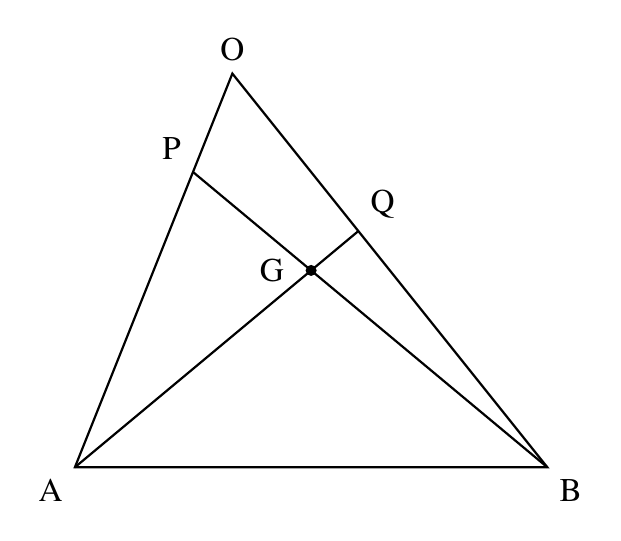
\begin{tikzpicture}\large
                \coordinate (o) at (0,0);
                \coordinate (a) at (-2,-5);
                \coordinate (b) at (4,-5);
                \draw[thick] (o)node[above]{O}--(a)node[below left]{A}--(b)node[below right]{B}--cycle;
                \draw[thick,name path=aq] (a)--($0.4*(b)$)node[above right]{Q};
                \draw[thick,name path=bp] (b)--($0.25*(a)$)node[above left]{P};
                \fill[name intersections={of=aq and bp,by={g}}](g)node[left=2mm]{G} circle (2pt);

                % \fill[red]($2/6*(a) + 2/3*(b)$) circle(2pt);
            \end{tikzpicture}

        \end{centering}

    \end{itembox}

    その気になれば,メネラウスの定理やチェバの定理を使うことで与えられた線分の長さの比から答えを導くことができる.しかし,ここではベクトルの一意性を用いて答えを求める.まず線分の比を自分で与える\footnote{線分AQ,BPに対して,その内分点Gに関する比を与える.与え方は自由だ.}.

    \begin{align*}
        \mathrm{AG}:\mathrm{GQ}&=s:1-s\\
        \mathrm{BG}:\mathrm{GP}&= t:1-t
    \end{align*}
    と与える.すると,
    \begin{align*}
        \overrightarrow{\mathrm{OG}}&=(1-s) \overrightarrow{\mathrm{OA}}
        +s \overrightarrow{\mathrm{OQ}}\\
        &= (1-s) \overrightarrow{\mathrm{OA}}
        + \frac{2}{5}s \overrightarrow{\mathrm{OB}}\\
        \overrightarrow{\mathrm{OG}} &= t \overrightarrow{\mathrm{OP}}
        +(1-t)\overrightarrow{\mathrm{OB}}\\
        &= \frac{1}{4}t \overrightarrow{\mathrm{OA}}
        +(1-t)\overrightarrow{\mathrm{OB}}
    \end{align*}
    となる.

    このように同一のベクトル \(\overrightarrow{\mathrm{OG}}\)が2通りの表現で表されている.また, \(\overrightarrow{\mathrm{OA}},\overrightarrow{\mathrm{OB}}\)は一次独立である.したがって,ベクトルの一意性より次の連立方程式を得る.
    \[
    \begin{cases}
        \displaystyle 1-s=\frac{1}{4}t\\
        \displaystyle\frac{2}{5}s=1-t
    \end{cases}
    \]
    連立方程式を解くと
    \[
    s=\frac{5}{6},\quad t=\frac{2}{3}
    \]
    となる.したがって
    \[
    \overrightarrow{\mathrm{OG}} = \frac{1}{6}\overrightarrow{\mathrm{OA}}+\frac{1}{3}\overrightarrow{\mathrm{{OB}}}
    \]
    となる.これで前半を答えたことになる.自ら線分の比を与え,それを連立方程式の利用によって求める.

    次は後半の部分で, \(OG\)を延長することを考える.このとき,3点O,G,Tは同一直線上にあることから,
    \[
    \overrightarrow{\mathrm{OT}}=k \overrightarrow{\mathrm{{OG}}}\qquad (k\text{は実数})
    \]
    とすることができる.この \(k\)を求めることができればよい.さらに条件として,3点A,T,Bは同一直線上にあるので,
    \[
    \overrightarrow{\mathrm{OT}}=x \overrightarrow{\mathrm{OA}}+y\overrightarrow{\mathrm{OB}}
    \]
    とすることができた場合,係数の和が \(x+y=1\)となる.したがって,
    \begin{align*}
        k\left(\frac{1}{6}+\frac{1}{3}\right)&=1\\
        &\Rightarrow k= 2\\
        \therefore \overrightarrow{\mathrm{OT}}&=\frac{1}{3}\overrightarrow{\mathrm{OA}}
        +\frac{2}{3}\overrightarrow{\mathrm{OB}}
    \end{align*}

    \subsection{図形の性質のベクトルによる確認}
    ベクトルの問題では数Aで学習した図形の持つ性質をベクトルを用いて再確認させるようなものがよくある.ある意味で当然なことを示すのだが,これが難しい場合がある.大抵,問題で与えられた図形の持つもともとの条件を忘れることが理由なので,落ち着いて問題にあたりたい.
    \begin{itembox}[l]{問題}
        \begin{enumerate}
            \item 正四面体において,交点を持たない2本の辺は垂直であることを示せ.
            \item 四面体ABCDにおいて, \(\mathrm{AC}\perp \mathrm{BD}\)ならば,
            \[
            \mathrm{AD}^2+\mathrm{BC}^2=\mathrm{AB}^2+\mathrm{CD}^2
            \]
            が成立することを示せ.
        \end{enumerate}
    \end{itembox}

    1問目は,つかみどころのないような問題文にしてみた.問題の様子を図\ref{tikz_sei_4_mentai}にする.例えば,赤線としてある2本の辺が交点を持たない辺の組である.正四面体において,この赤線の辺の組は垂直であるのだ.
    \begin{figure}[htbp]\centering
        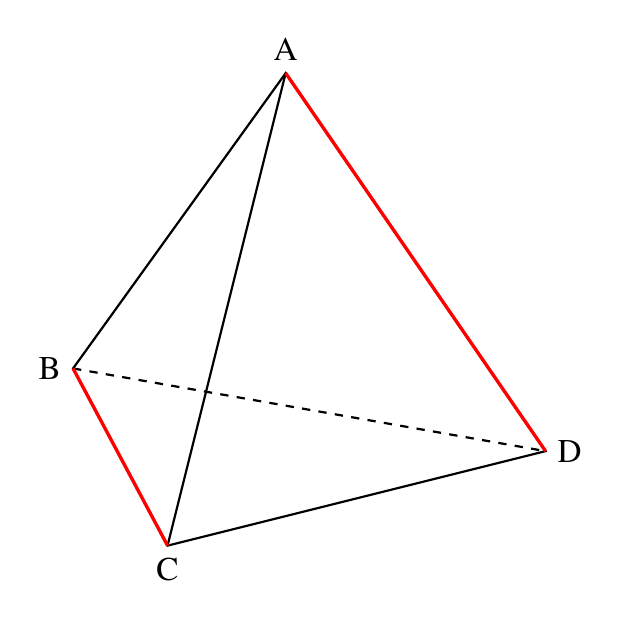
\begin{tikzpicture}[scale=1.5]\large
            \coordinate (a) at (1,4);
            \coordinate (b) at (-0.8,1.5);
            \coordinate (c) at (0,0);
            \coordinate (d) at (3.2,0.8);
            \draw[thick](a)node[above]{A}--(b)node[left]{B}--(c)node[below]{C}--(d)node[right]{D}--cycle;
            \draw[thick](a)--(c);
            \draw[thick,dashed](b)--(d);
            \draw[red,very thick](b)--(c);
            \draw[red,very thick](a)--(d);
        \end{tikzpicture}
        \caption{正四面体}
        \label{tikz_sei_4_mentai}
    \end{figure}

    解法の手順としては,正四面体の頂点のどれかを定点とした位置ベクトルを置くことから始まる.また,頂点の名前は自由における状態であるということは,1つの辺の組さえ証明してしまえば,図形の対称性から残りは自明となることを利用する.証明問題なので,厳密に解答する.

    \begin{proof}
        図\ref{tikz_sei_4_mentai}の正四面体において,点Aを始点とした位置ベクトルを考え,残りの3点は位置ベクトルで \(\vec{b},\vec{c},\vec{d}\)と表すことにする.正四面体であるという条件から,すべての辺の長さは等しく,また,隣り合った2辺のなす角は60度である.したがって,
        \[
        \vec{b}\cdot\vec{c}=\vec{c}\cdot\vec{d}=\vec{d}\cdot\vec{b}
        \]
        である.

        これを用いると,
        \begin{align*}
            \vec{d}\cdot(\vec{b}-\vec{c})&= \vec{d}\cdot\vec{b}-\vec{d}\cdot\vec{c}\\
            &=0\\
            \therefore \mathrm{AD}&\perp \mathrm{BC}
        \end{align*}
        と分かる.つまり,交点を持たない2本の辺の組の1つであるAD,BCで題意を示したことになる.さらに,図形の対称性より,同様の議論を繰り返すことで,すべての交点を持たない2本の辺の組で題意を示すことができる.

    \end{proof}

    2問目は立体の図形的な情報を辺の長さという数値の情報に変換する問題だ.図\ref{tikz_simentai}の赤い部分が垂直であるのが条件である\footnote{図の使いまわし,すみません.}.

    \begin{figure}[htbp]\centering
        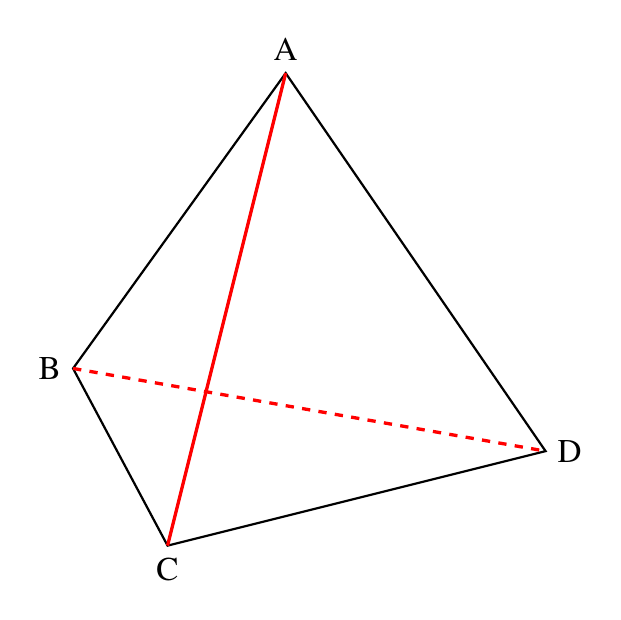
\begin{tikzpicture}[scale=1.5]\large
            \coordinate (a) at (1,4);
            \coordinate (b) at (-0.8,1.5);
            \coordinate (c) at (0,0);
            \coordinate (d) at (3.2,0.8);
            \draw[thick](a)node[above]{A}--(b)node[left]{B}--(c)node[below]{C}--(d)node[right]{D}--cycle;
            \draw[thick](a)--(c);
            \draw[red ,very thick,dashed](b)--(d);
            \draw[red,very thick](a)--(c);
        \end{tikzpicture}
        \caption{正四面体}
        \label{tikz_simentai}
    \end{figure}

    \begin{proof}

        図\ref{tikz_simentai}の正四面体において,点Aを始点とした位置ベクトルを考え,残りの3点は位置ベクトルで \(\vec{b},\vec{c},\vec{d}\)と表すことにする.
        問題の条件より \(\mathrm{AC}\perp \mathrm{BD}\)なので,
        \begin{align*}
            \vec{c}\cdot (\vec{d}-\vec{b})&= \vec{c}\cdot\vec{d}-\vec{c}\cdot\vec{b}\\
            &=0\\
            \therefore \vec{c}\cdot\vec{b}&=\vec{c}\cdot\vec{d}
        \end{align*}

        さて,ここで示すべき式の左辺をベクトルで計算する.
        \begin{align*}
            (\text{左辺})&=|\vec{d}|^2 +|\vec{c}-\vec{b}|^2\\
            &=|\vec{b}|^2 +|\vec{c}|^2 +|\vec{d}|^2 -2\vec{c}\cdot\vec{b}
        \end{align*}
        同様に右辺もベクトルで計算する.
        \begin{align*}
            (\text{右辺})&=|\vec{b}|^2+|\vec{d}-\vec{c}|^2\\
            &=|\vec{b}|^2 +|\vec{c}|^2 +|\vec{d}|^2 -2\vec{c}\cdot\vec{d}
        \end{align*}
        \(\vec{c}\cdot\vec{b}=\vec{c}\cdot\vec{d}\)より \((\text{左辺})=(\text{右辺})\)
    \end{proof}

    






\end{document}


    \chapter{ベクトル方程式}
    ベクトルと変数(スカラ量)を用いて図形を表現することをベクトル方程式という.発展的な内容であり,問題の解法の1つとして使えるものだ.しかし,優先度は高くなく,ベクトル方程式を利用できる問題は他の解法でも解ける.
\newpage

    \documentclass[dvipdfmx]{jsarticle}
\usepackage{graphics}
\usepackage{amsmath}
\usepackage{amssymb}
\usepackage{amsthm}
\usepackage{mathtools}
\usepackage{ascmac}
\usepackage{bm}
\usepackage{url}
\usepackage{txfonts}
\usepackage{color}
\usepackage{tikz}
% \usepackage{docmute}    %パッケージのダウンロードが必要
\usepackage{tikz}
\usetikzlibrary{calc}
\usetikzlibrary{intersections}

\begin{document}
    \section{ベクトル方程式の導入}
    原点を始点とし,成分が(1,0)となるベクトル \(\vec{x}\)をとる.するとxy平面において,x軸上の任意の点は \(t\vec{x},(t\text{は実数})\)というベクトルで表現できる.これはx軸という直線がベクトルと実数の積で表現されたということができる.このように,空間上の点や直線,面などをベクトルと実数で表すのがベクトル方程式だ.以下,代表的なベクトル方程式を紹介する.

    \section{直線のベクトル方程式}
    \subsection{位置と方向1}

    直線のベクトル方程式で必要なのは,直線の進む方向(傾き)と直線の位置(直線の通過する1点)だ.1次関数が傾きとy切片で決定することに似ている.定点Oをとり,点A,Bを通る直線を考えると,そのベクトル方程式 \(\vec{p}\)\footnote{ベクトル方程式を考えるときに,表現する図形上の点をPとし,そのベクトルを \(\vec{p}\)とするのは慣習である.}は
    \[
    \vec{p}=\vec{a} + t(\vec{b}-\vec{a})\qquad t:\text{実数}
    \]
    となる(図\ref{tikz_vector_equation_line1}).

    \begin{figure}[htbp]\centering
        \begin{tikzpicture}\large
            \coordinate (o) at (0,0);
            \coordinate (a) at (-1,2);
            \coordinate (b) at (2,3);

            \fill (o)node[below]{O} circle (2pt);
            \fill (a)node[above]{A} circle (2pt);
            \fill (b)node[above]{B} circle (2pt);

            \draw ($(a)  -(b)+(a)$) -- ($(a) + 2*(b) - 2*(a)$);

            \draw[red,thick,->](o)--node[left]{\(\vec{a}\)}(a);
            \draw[red,thick,->](a)--node[below]{\(t(\vec{b}-\vec{a})\)}($1/3*(a)+2/3*(b)$);
            \fill[red] ($1/3*(a)+2/3*(b)$)node[above]{P} circle(2pt);

        \end{tikzpicture}
        \caption{直線のベクトル方程式1}
        \label{tikz_vector_equation_line1}
    \end{figure}

    \(t\)を自由に変化させることで直線AB上を点Pが動くことがわかる.ここからは直線のベクトル方程式を一般化する.まずは直線の位置を表す部分だ. \(\vec{a}\)によって直線と点Oの位置関係が決定している.だが,これは直線上の1点であれば何でもよい.図のようなベクトルを考え,
    \[
    \vec{p}=\vec{c} + t(\vec{b}-\vec{a})\qquad t:\text{実数}
    \]
    としても良い.

    \begin{figure}[htbp]\centering
        \begin{tikzpicture}\large
            \coordinate (o) at (0,0);
            \coordinate (a) at (-1,2);
            \coordinate (b) at (2,3);
            \coordinate (c) at ($5/4*(a)-1/4*(b)$);

            \fill (o)node[below]{O} circle (2pt);
            \fill (a)node[above]{A} circle (2pt);
            \fill (b)node[above]{B} circle (2pt);
            \fill (c)node[above]{C} circle (2pt);

            \draw ($(a)  -(b)+(a)$) -- ($(a) + 2*(b) - 2*(a)$);

            \draw[red,thick,->](o)--node[left]{\(\vec{c}\)}(c);
            \draw[red,thick,->](c)--node[below]{\(t(\vec{b}-\vec{a})\)}($1/3*(a)+2/3*(b)$);
            \fill[red] ($1/3*(a)+2/3*(b)$)node[above]{P} circle(2pt);

        \end{tikzpicture}
        \caption{直線のベクトル方程式2}
        \label{tikz_vector_equation_line1_sub1}
    \end{figure}

    もちろん,直線の位置を示すベクトルが \(\vec{a}\)から \(\vec{c}\)に変わっているので,同じ点Pを表現しようと思うと, \(t\)の値が変わる.しかし,直線を表現しているという点では何ら変化はない.


    次に一般化するのは直線の方向を示すベクトルだ.今の例では \(\vec{b}-\vec{a}\)が方向を示すベクトルとなっているが,これは実数倍で自由\footnote{自由とは,変更が可能であるということである. \(t(\vec{b}-\vec{a})=t/2\cdot 2(\vec{b}-\vec{a})\)であるから方向を表すベクトルを \(2(\vec{b}-\vec{a})\)に変更しても問題はない.}だ.そこで方向を示すベクトルは \(\vec{b}-\vec{a}\)に平行な何らかのベクトル \(\vec{d}\)であるとする.

    以上から一般的な直線のベクトル方程式は
    \begin{equation}
        \vec{p}=\vec{c}+t\vec{d}\qquad t:\text{実数}
        \label{eq_vector_equation_line1}
    \end{equation}
    とすることができる\footnote{変化しない定ベクトルをconstant vector,方向ベクトルをdirection vectorと呼び,そこから \(\vec{c},\vec{d}\)としていたりもする.}.直線のベクトル方程式を求めるとは, \(\vec{c},\vec{d}\)を求めることである.もちろん2次元,3次元で同じように扱える公式である.

    \subsection{位置と方向2}
    前項では方向を直接に表現していた. \(\vec{d}\)によって方向を決定し \(t\)倍していた.ベクトルの世界では"同じ方向"と同じくらい特殊な方向の関係がある.それは"垂直"であり,本項では直線の方向を,その法線で与えられている場合を考える.

    図\ref{tikz_vector_equation_line2}のように法線ベクトル \(\vec{n}\)\footnote{法線ベクトルはnormal vectorと呼ぶ.そのため法線ベクトルは \(\vec{n}\).}と,直線上の一点が与えられているとする.すると直線上の任意の点Pをとることで次の式を立てることができる.
    \begin{equation}
        \vec{n}\cdot(\vec{p}-\vec{c})=0
        \label{eq_vector_equation_line2}
    \end{equation}
    これがベクトル方程式なのだ.式\eqref{eq_vector_equation_line1}とは異なり,変数 \(t\)がない.そのため,直線上の1点を決定することはできない.だが, \(\vec{p}\)は直線上のすべての点になり得ることになり,直線全体を表すベクトル方程式であるということができる.

    \begin{figure}[htbp]\centering
        \begin{tikzpicture}\large
            \coordinate (o) at (0,0);
            \coordinate (c) at (-1,2);
            \coordinate (p) at (2,3);
            \coordinate (n) at ($(c)!0.5!(p)$);

            \fill (o)node[below]{O} circle (2pt);
            \fill (a)node[above]{A} circle (2pt);

            \draw ($(c)!-1!(p)$)--($(c)!2!(p)$);
            \draw[red,thick,->] (n)--node[above right]{\(\vec{n}\)}($(n)!1cm!90:(p)$);
            \draw[red,thick,->] (c)--node[below right]{\(\vec{p}-\vec{c}\)}(p)node[above]{P};

        \end{tikzpicture}
        \caption{直線のベクトル方程式3}
        \label{tikz_vector_equation_line2}
    \end{figure}

    理解が難しいのは \(\vec{p}\)が決定しないからだ.ベクトル方程式というのは,図形のある1点をPとしたときに
    \[
    \vec{p}=(\text{条件式})
    \]
    という風に点を決定するものではなく,図形のすべての点Pに対して \(\vec{p}\)が満たす式である.このことを念頭に話を進める.

    \section{円のベクトル方程式}
    \subsection{中心と半径}
    円とは,半径から等距離に存在する点の集合だ.そこで円の中心を示す位置ベクトルを \(\vec{c}\),半径を \(r\)とすると,円周上のすべての \(\vec{p}\)は
    \begin{equation}
        |\vec{p}-\vec{c}|=r
        \label{eq_vector_equation_circle1}
    \end{equation}
    を満たす.これが円のベクトル方程式なのだ.図\ref{tikz_vector_equation_circle1}がその参考となる図である.

    \begin{figure}[htbp]\centering
        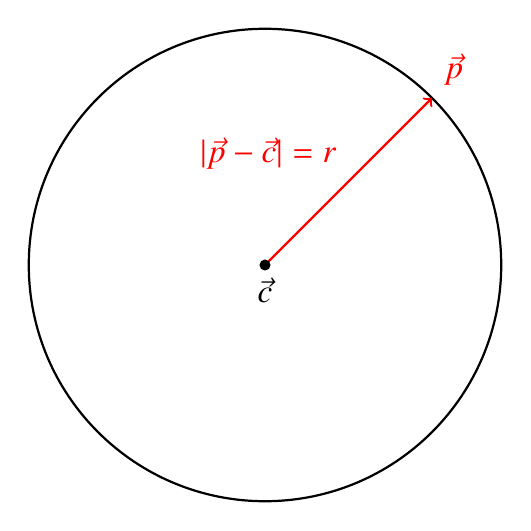
\begin{tikzpicture}\large
            \coordinate (o) at (0,0);
            \coordinate (p) at (45:3);

            \draw[thick] (o)node[below]{\(\vec{c}\)} circle[radius=3];
            \draw[red,thick,->](o)--node[above left]{\(|\vec{p}-\vec{c}|=r\)}(p)node[above right]{\(\vec{p}\)};
            \fill (o) circle (2pt);

        \end{tikzpicture}
        \caption{円のベクトル方程式}
        \label{tikz_vector_equation_circle1}
    \end{figure}

    \subsection{直径}
    線分ABを直径とする円を考える.この場合のベクトル方程式を考えるときに利用するのは,直径の円周角が90度であることだ.直角であればベクトルの内積が0になるので,ここからベクトル方程式を立てることができる.

    線分の両端の位置ベクトルを \(\vec{a},\vec{b}\)とすると,円のベクトル方程式は
    \begin{equation}
        (\vec{p}-\vec{a})\cdot(\vec{p}-\vec{b})=0
        \label{eq_vector_equation_circle2}
    \end{equation}
    となる.次のようなイメージとなる(図\ref{tikz_vector_equation_circle2}).

    \begin{figure}[htbp]\centering
        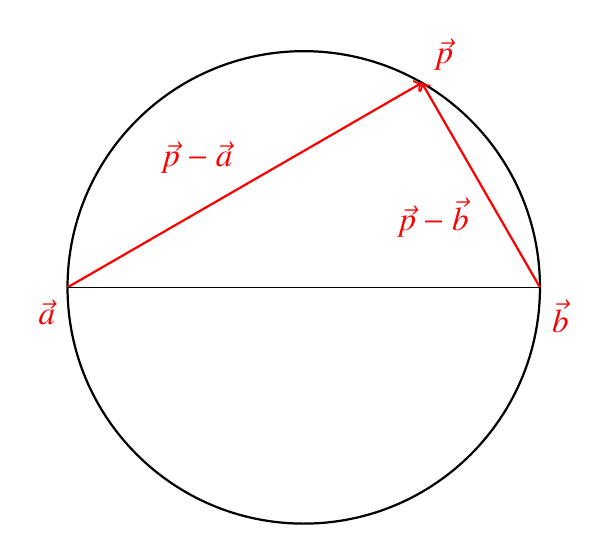
\begin{tikzpicture}\large
            \coordinate (o) at (0,0);
            \coordinate (a) at (-3,0);
            \coordinate (b) at (3,0);
            \coordinate (p) at (60:3);

            \draw[thick](o)circle[radius=3];
            \draw[red,thick,->](a)node[below left]{\(\vec{a}\)}--node[above left]{\(\vec{p}-\vec{a}\)}(p)node[above right]{\(\vec{p}\)};
            \draw[red,thick,->](b)node[below right]{\(\vec{b}\)}--node[below left]{\(\vec{p}-\vec{b}\)}(p);

            \draw (a)--(b);
        \end{tikzpicture}
        \caption{円のベクトル方程式}
        \label{tikz_vector_equation_circle2}
    \end{figure}

    点PがもしA,Bと一致しても式\eqref{eq_vector_equation_circle2}を満たすので心配はない.2つの円のベクトル方程式を紹介したが,どちらも円周上の1点を決定するものではない.

    \section{平面のベクトル方程式}
    \subsection{位置と平面}
    一次独立な2つのベクトルがあれば,その2つのベクトルが属する平面の任意の点を示すことができる.これは前章で扱った内容だ.そして,それと平面の位置を決定する要素があれば,3次元空間に1つの平面を決定することができる.

    今の表現は難解なので,具体例を示す.図のように,基準となる定点Oと3点A,B,Cをとる.すると,3点A,B,Cによって決定する平面のベクトル方程式は次のようになる.
    \[
    \vec{p}=\vec{a} + s(\vec{b}-\vec{a})+t(\vec{c}-\vec{a})\qquad s,t:\text{実数}
    \]

    \begin{figure}[htbp]\centering
        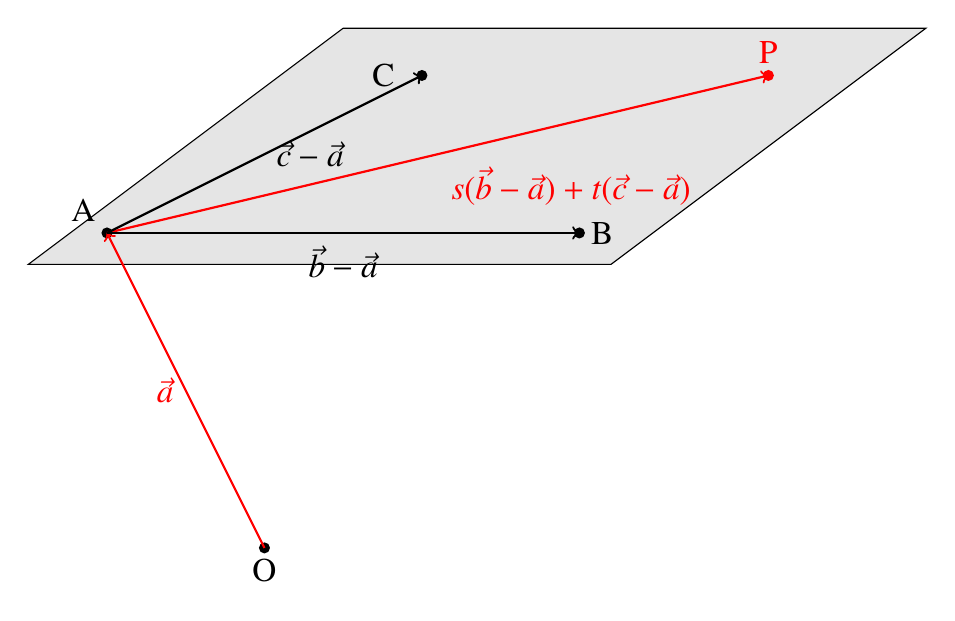
\begin{tikzpicture}[scale=2]\large
            \coordinate (o) at (0,0);
            \coordinate (a) at (-1,2);
            \coordinate (b) at (2,2);
            \coordinate (c) at (1,3);
            \coordinate (p) at (3.2,3);

            \filldraw[fill=black!10,draw=black,thin] (-1.5,1.8)--(2.2,1.8)--(4.2,3.3)--(0.5,3.3)--cycle;
            \fill (o)node[below]{O} circle(1pt);
            \fill (a)node[above left]{A} circle(1pt);
            \fill (b)node[right]{B} circle(1pt);
            \fill (c)node[left=2mm]{C} circle(1pt);
            \fill[red] (p)node[above]{P} circle(1pt);

            \draw[red,thick,->](o)--node[left]{\(\vec{a}\)}(a);
            \draw[red,thick,->](a)--node[below right]{\(s(\vec{b}-\vec{a})+t(\vec{c}-\vec{a})\)}(p);

            \draw[thick,->](a)--node[below]{\(\vec{b}-\vec{a}\)}(b);
            \draw[thick,->](a)--node[right]{\(\vec{c}-\vec{a}\)}(c);
        \end{tikzpicture}
        \caption{平面のベクトル方程式1}
        \label{tikz_vector_equation_plane1}
    \end{figure}

    直線のベクトル方程式と同じように一般化を考える.面の一点を示す位置ベクトルを \(\vec{c}\)\footnote{図\ref{tikz_vector_equation_plane1}の \(\vec{c}\)とは別物.定ベクトル.}とし,さらに示したい平面に属する一次独立はベクトルの組を \(\vec{k},\vec{l}\)とすると,平面のベクトル方程式は,
    \begin{equation}
        \vec{p} =\vec{c} +s\vec{k}+t\vec{l}\qquad s,t:\text{実数}
        \label{eq_vector_equation_plane1}
    \end{equation}
    となる.

    \subsection{位置と法線}
    直線と同様で,平面のベクトル方程式でも法線ベクトルを考えることができる.面の法線とは面のいかなる線分に対しても垂直な直線のことである.ここから法線ベクトル \(\vec{n}\)は面に属する一次独立な2本のベクトルの両方と垂直なベクトルとすることができる.法線ベクトルと,平面上の1点 \(\vec{c}\)によってベクトル方程式は
    \begin{equation}
        \vec{n}\cdot (\vec{p}-\vec{c})=0
        \label{eq_vector_equation_plane2}
    \end{equation}
    となる(図\ref{tikz_vector_equation_plane2}).

    \begin{figure}[htbp]\centering
        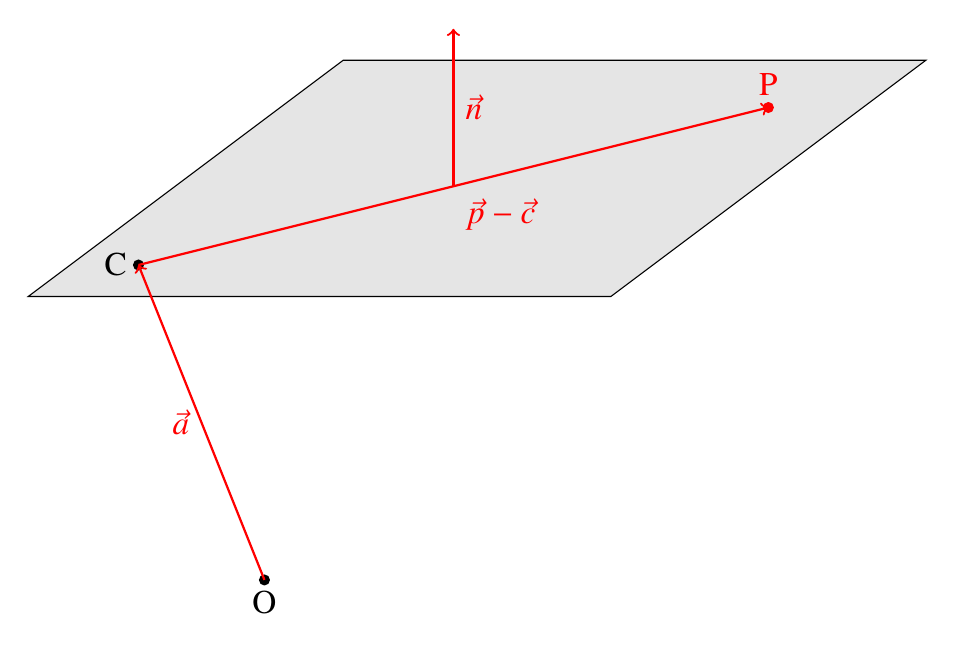
\begin{tikzpicture}[scale=2]\large
            \coordinate (o) at (0,0);
            \coordinate (c) at (-0.8,2);
            \coordinate (p) at (3.2,3);

            \filldraw[fill=black!10,draw=black,thin] (-1.5,1.8)--(2.2,1.8)--(4.2,3.3)--(0.5,3.3)--cycle;
            \fill (o)node[below]{O} circle(1pt);
            \fill (c)node[left]{C} circle(1pt);
            \fill[red] (p)node[above]{P} circle(1pt);

            \draw[red,thick,->](o)--node[left]{\(\vec{a}\)}(c);
            \draw[red,thick,->](c)--node[below right]{\(\vec{p}-\vec{c}\)}(p);

            \draw[red ,thick,->]($(c)!0.5!(p)$)--node[right]{\(\vec{n}\)}($(c)!0.5!(p) + (90:1)$);

        \end{tikzpicture}
        \caption{平面のベクトル方程式2}
        \label{tikz_vector_equation_plane2}
    \end{figure}

    平面上のすべての \(\vec{p}\)で式\eqref{eq_vector_equation_plane2}が成立する.ことからこれはベクトル方程式である.

    \section{球のベクトル方程式}
    これは円のベクトル方程式を3次元に拡張したものだ.中心の座標を \(\vec{c}\),半径を \(r\)とすると,
    \begin{equation}
        |\vec{p}-\vec{c}|=r
        \label{eq_vector_equation_ball1}
    \end{equation}
    となる.これは式\eqref{eq_vector_equation_circle1}と全く同じ式だ.

    さらに,球の直径の両端がわかるときにベクトル方程式は式\eqref{eq_vector_equation_circle2}と同じで,
    \begin{equation}
        (\vec{p}-\vec{a})\cdot(\vec{p}-\vec{b})=0
        \label{eq_vector_equation_ball2}
    \end{equation}
    となる.

    \section{ベクトル方程式と座標系}
    ベクトル方程式において,そのベクトルの成分が明らかなとき,座標系の関数に直すことができる.媒介変数表示というものの理解が必要だ.
    \subsection{直線のベクトル方程式と座標系}
    直線のベクトル方程式である式\eqref{eq_vector_equation_line1}において,
    \[
    \begin{cases}
        \vec{c}&=(1,2)\\
        \vec{d}&=(3,2)
    \end{cases}
    \]
    とする.直線上の点を \(\vec{p}=(x,y)\)とすると,ベクトル方程式から
    \begin{align*}
        (x,y)&= (1,2)+t(3,2)\\
        \Rightarrow &\begin{cases}
            x&= 3t+1\\
            y&=2t+2
        \end{cases}
    \end{align*}
    と分かる.これは媒介変数 \(t\)の媒介変数表示である.さらに,媒介変数を消去することで,
    \[
    2x-3y=4\Rightarrow y=\frac{2}{3}x- \frac{4}{3}
    \]
    を得る.これで直線のベクトル方程式を1次関数にすることができた.

    次は式\eqref{eq_vector_equation_line2}の形のベクトル方程式を求める.法線ベクトル \(\vec{n}\)は \(\vec{d}\)に垂直なベクトルとして与えられる.そこから,内積を計算することで求めることができる.そのほかにも求める方法があり,直線の方程式
    \[
    2x-3y=-4
    \]
    から, \(x,y\)の係数を取り出すことで \(\vec{n}=(2,-3)\)とすることもできる.これは偶然ではない.ともあれ,法線ベクトルは \(\vec{n}=(2,-3)\)として得ることができた.また,直線上の1点は \((1,2)=\vec{c}\)をそのまま使い,
    \[
    \vec{n}\cdot(\vec{p}-\vec{c})=0
    \]
    を得る\footnote{ベクトルの内積の表記において, \((1,2)\cdot(4,5)\)というような成分表示されたベクトルを使うのは誤りである.これは大学の数学を学ぶときに明らかになるが,ここでは詳しく述べない.}.

    以上で,直線のベクトル方程式と座標系の関連が明らかになった.さらに1次関数の一般形\footnote{\(ax+by+c=0\)という表記をした1次関数を1次関数の一般形という.}から,直線の法線ベクトルを得られることも分かった.

    \subsection{円のベクトル方程式と座標系}
    式\eqref{eq_vector_equation_circle1}を \(\vec{p}=(x,y),\vec{c}=(a,b)\)として計算する.
    \begin{align*}
        |\vec{p}-\vec{c}|&= r\\
        {\color{red} \Leftrightarrow} |\vec{p}-\vec{c}|^2&= r^2\qquad {\color{red}(\because \text{両辺は同符号})}\\
        (x-a)^2+(y-b)^2&=r^2
    \end{align*}
    得られた式は中心が \((a,b)\),半径が \(r\)の円の式である.赤字の部分はなくても良いが,2乗すると基本的に同値ではなくなる\footnote{\((-1)^2=1^2\)より2乗が等しいから,2乗する前が等しいとは限らない.これを意識した記述が必要な時がある.}ことに注意しよう.

    式\eqref{eq_vector_equation_circle2}についても同様の計算をする. \(\vec{a}=(x_a,y_a),\vec{b}=(x_b,y_b)\)とする.
    \begin{align*}
        (\vec{p}-\vec{a})\cdot(\vec{p}-\vec{b})&= (x-x_a)(x-x_b) +(y-y_a)(y-y_b)\\
        &= \{x^2-(x_a+x_b)x+x_ax_b\} +\{y^2-(y_a+y_b)y+y_ay_b\}\\
        &= \left( x- \frac{x_a+x_b}{2} \right)^2 - \frac{1}{4}x_a^2+\frac{1}{2}x_ax_b -\frac{1}{4}x_b^2
        +\left( y- \frac{y_a+y_b}{2} \right)^2 -\frac{1}{4}y_a^2 +\frac{1}{2}y_ay_b -\frac{1}{4}y_b^2\\
        &=0\\
        \therefore &\left( x- \frac{x_a+x_b}{2} \right)^2
        +\left( y- \frac{y_a+y_b}{2} \right)^2
        = \left( \frac{x_a-x_b}{2} \right)^2 +\left( \frac{y_a-y_b}{2} \right)^2
    \end{align*}
    得られる式は直径の中点を中心とした直径の半分の長さを半径とする円の式である.

    以上から円のベクトル方程式と座標系の関係が明らかになった.

    \subsection{ベクトル方程式と3次元座標系}
    ベクトル方程式をわざわざ3次元座標系の関数に直すことはまずない.これはベクトルの導入によって3つの要素を扱うべき空間図形の問題を大きさ,向きの2つの要素に変換するというベクトルの有用性によるものだ.せっかくの利点を損なうことはない.

    しかし,容易に計算できるもののみを紹介する.
    まずは球面の方程式だ.これは式\eqref{eq_vector_equation_ball1}において \(\vec{c}=(a,b,c)\)とすることで計算される.
    \begin{equation}
        (x-a)^2+(y-b)^2+(z-c)^2=r^2
    \end{equation}
    これは中心が \((a,b,c)\)で半径が \(r\)の球面の公式である.

    続いて平面の公式である.これは法線を利用した式\eqref{eq_vector_equation_plane2}において法線ベクトルを \(\vec{n}=(a,b,c)\),平面上の1点を \(\vec{c}=(x_1,y_1,z_1)\)とすることで得られる.
    \begin{equation}
        a(x-x_1)+b(y-y_1)+c(z-z_1)=0
    \end{equation}

    これら2式は公式として丸覚えすればいい.


    \section{ベクトル方程式の利用}
    ベクトル方程式は求めたいベクトルの条件式の1つとして利用することが多い.例として次の問題をベクトル方程式を利用して解いてみる.
    \begin{itembox}[l]{問題}
        中心 \((1,2)\),半径4の円周上のとる点をPとする.線分OPとx軸の正の方向とのなす角が45度となるPがあれば,すべて挙げよ.
    \end{itembox}
    このような問題ではベクトルを使う解法はとらない.しかし,できないことはない.

    早速,解答に移る.解答に用いる位置ベクトルの始点は原点とする.点Pの位置ベクトル \(\vec{p}\)は条件の円周上にあるので以下のベクトル方程式を満たす.
    \[
    |\vec{p}-\vec{c}|=4\qquad \vec{c}=(1,2)
    \]
    さらに \(\vec{p}\)はx軸の正方向とのなす角が45度なので, \(\vec{x}=(1,0)\)をとると,
    \[
    \vec{p}\cdot\vec{x}=|\vec{p}|\cos45^\circ = x_p\qquad x_p:\vec{p}\text{のx成分}
    \]

    得られた2式に対して \(\vec{p}=(x_p,y_p)\)を代入することで
    \[
    \begin{cases}
        |(x_p-1,y_p-2)|&=4\\
        \displaystyle\frac{|(x_p,y_p)|}{\sqrt{2}}&=x_p
    \end{cases}
    \]
    という連立方程式を得る.2つ目の式を計算すると
    \begin{align*}
        x_p^2+y_p^2&=2x_p^2\\
        \therefore y_p&=\pm x_p
    \end{align*}
    ここからは場合分けをする. \(x_p=y_p\)のとき,
    \begin{align*}
        (x_p-1)^2+(x_p-2)^2&= 16\\
        \Leftrightarrow 2x_p^2 -6 x_p-9&=0\\
        \therefore x&= \frac{3\pm3\sqrt{3}}{2}(=y_p)
    \end{align*}
    \(-x_p=y_p\)のとき,
    \begin{align*}
        (x_p-1)^2+(-x_p-2)^2&= 16\\
        \Leftrightarrow 2x_p^2 +2 x_p-9&=0\\
        \therefore x&= \frac{-1\pm\sqrt{19}}{2}(=-y_p)
    \end{align*}
    となる.結局4つのPが存在したことになる.これを図\ref{tikz_vector_equation_example_question}で確認する.x軸の正方向となす角が45度とは,結局のところ \(y=x,y=-x\)のことを意味している.

    \begin{figure}[htbp]\centering
        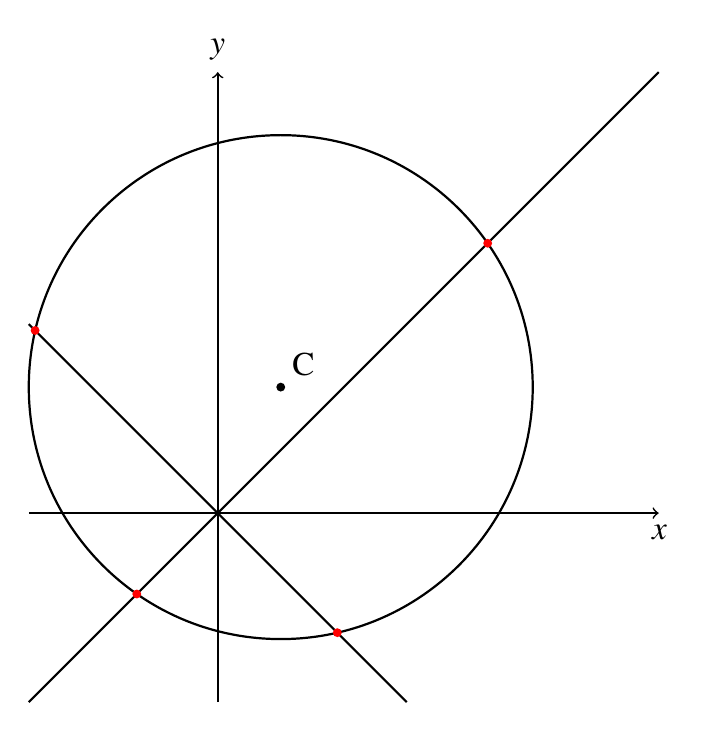
\begin{tikzpicture}[scale=0.8]\large
            \coordinate (c) at (1,2);
            \draw[semithick,->](-3,0)--(7,0)node[below]{\(x\)};
            \draw[semithick,->](0,-3)--(0,7)node[above]{\(y\)};
            \fill (c)node[above right]{C} circle (2pt);
            \draw[thick,name path=c_circ](c)circle[radius=4];
            \draw[thick,name path=p_x](-3,-3)--(7,7);
            \draw[thick,name path=m_x](-3,3)--(3,-3);

            \fill[name intersections={of=c_circ and p_x,by={p1,p2}},red] (p1) circle(2pt);
            \fill[red](p2)circle (2pt);
            \fill[name intersections={of=c_circ and m_x,by={m1,m2}},red] (m1) circle(2pt);
            \fill[red](m2)circle (2pt);

        \end{tikzpicture}
        \caption{問題の結果}
        \label{tikz_vector_equation_example_question}
    \end{figure}


    この例からもわかる通り,ベクトル方程式は求めたいベクトルの条件を与えるために用いられる.そのため,"方程式"なのだ.
    そして,これは無意識のうちになされることが多く,さらには条件の与え方を方程式という形ではなく,ベクトルの成分として
    \footnote{本問では,容易に \(y=\pm x\)が得られるので,計算をする前から \(\vec{p}=(x,x),(x,-x)\)とおいて, \(x\)についての計算問題とするほうが自然だ.}
    与えるケースが多い.そのため,優先度の低い事柄となっている.発想としては重要なものであるのでマスターしたい.\\

    ベクトル方程式の章では問題を用意しない.これまでの問題や,問題集の問題をベクトル方程式を用いて解くことで復習してほしい.

    \section*{まとめ}
    数B:ベクトルの内容を計算,図形,方程式という3つの側面から扱った.その中でもベクトルの有効性を発揮するために重要なのは,内積などの特別な計算規則を身につけることだ.ベクトルという大きさと向きを持つ量が,計算規則に従うことであたかも文字式のように扱えるようになることが極めて重要なことである.

    図形では,本来3つの要素を取り扱わなければならない3次元の問題に対しても代数的な計算を実現している.これがベクトルの最大の利点である.しかし,いかなる状況でもベクトルが有効なのではなく,角度や大きさが前面に出る問題では計算を実行できないというケースが存在するので,使いどころには注意が必要だ.これに関しては,反復練習のみが有効な訓練となる.

    最後のベクトル方程式はベクトルを図形に反映させるための1通りの手法ととらえると,良いだろう.ベクトルを求めるときに,ベクトルの成分を未知数として考えるのは良くない.それは単なる計算問題となってしまう.しかし,ベクトル方程式を立て,未知のベクトルを直接求めようとすれば,さらにベクトルの有効性を体感するに至るだろう.











\end{document}


    \vspace{5mm}
    以上.

    \newpage
    \documentclass[dvipdfmx]{jsarticle}
\usepackage{graphics}
\usepackage{amsmath}
\usepackage{amssymb}
\usepackage{amsthm}
\usepackage{mathtools}
\usepackage{ascmac}
\usepackage{bm}
\usepackage{url}
\usepackage{txfonts}
\usepackage{color}
\usepackage{tikz}
% \usepackage{docmute}    %パッケージのダウンロードが必要
\usepackage{tikz}
\usetikzlibrary{calc}
\usetikzlibrary{intersections}

\begin{document}
    \section*{最後に}
    本資料は以下のURLのサイトに掲載されているものです.

    {\centering \url{https://blkdenden.firebaseapp.com/lib.html}\\}

    転載などはしないでください.

    また,誤植などは順次訂正しますが,不明な点は掲載サイトのコンタクト欄からメールを送信,または以下のメールアドレスに問い合わせてください.

    {\centering \url{s.kondo11235813@gmail.com}\\}

    % \section*{参考文献}
    % \begin{itemize}
    %     \item 『高等学校 数学B』,数研出版(2017)
    % \end{itemize}




\end{document}



\end{document}
